%Version 3.1 December 2024
% See section 11 of the User Manual for version history
%
%%%%%%%%%%%%%%%%%%%%%%%%%%%%%%%%%%%%%%%%%%%%%%%%%%%%%%%%%%%%%%%%%%%%%%
%%                                                                 %%
%% Please do not use \input{...} to include other tex files.       %%
%% Submit your LaTeX manuscript as one .tex document.              %%
%%                                                                 %%
%% All additional figures and files should be attached             %%
%% separately and not embedded in the \TeX\ document itself.       %%
%%                                                                 %%
%%%%%%%%%%%%%%%%%%%%%%%%%%%%%%%%%%%%%%%%%%%%%%%%%%%%%%%%%%%%%%%%%%%%%

%%\documentclass[referee,sn-basic]{sn-jnl}% referee option is meant for double line spacing

%%=======================================================%%
%% to print line numbers in the margin use lineno option %%
%%=======================================================%%

%%\documentclass[lineno,pdflatex,sn-basic]{sn-jnl}% Basic Springer Nature Reference Style/Chemistry Reference Style

%%=========================================================================================%%
%% the documentclass is set to pdflatex as default. You can delete it if not appropriate.  %%
%%=========================================================================================%%

%%\documentclass[sn-basic]{sn-jnl}% Basic Springer Nature Reference Style/Chemistry Reference Style

%%Note: the following reference styles support Namedate and Numbered referencing. By default the style follows the most common style. To switch between the options you can add or remove “Numbered” in the optional parenthesis. 
%%The option is available for: sn-basic.bst, sn-chicago.bst%  
 
%%\documentclass[pdflatex,sn-nature]{sn-jnl}% Style for submissions to Nature Portfolio journals
%%\documentclass[pdflatex,sn-basic]{sn-jnl}% Basic Springer Nature Reference Style/Chemistry Reference Style
% \documentclass[pdflatex,sn-mathphys-num]{sn-jnl}% Math and Physical Sciences Numbered Reference Style
%%\documentclass[pdflatex,sn-mathphys-ay]{sn-jnl}% Math and Physical Sciences Author Year Reference Style
%%\documentclass[pdflatex,sn-aps]{sn-jnl}% American Physical Society (APS) Reference Style
%%\documentclass[pdflatex,sn-vancouver-num]{sn-jnl}% Vancouver Numbered Reference Style
%%\documentclass[pdflatex,sn-vancouver-ay]{sn-jnl}% Vancouver Author Year Reference Style
\documentclass[pdflatex,sn-apa]{sn-jnl}% APA Reference Style
%%\documentclass[pdflatex,sn-chicago]{sn-jnl}% Chicago-based Humanities Reference Style

%%%% Standard Packages
%%<additional latex packages if required can be included here>

\usepackage{graphicx}%
\usepackage{multirow}%
\usepackage{amsmath,amssymb,amsfonts}%
\usepackage{amsthm}%
\usepackage{mathrsfs}%
\usepackage[title]{appendix}%
\usepackage{xcolor}%
\usepackage{textcomp}%
\usepackage{manyfoot}%
\usepackage{booktabs}%
\usepackage{algorithm}%
\usepackage{algorithmicx}%
\usepackage{algpseudocode}%
\usepackage{listings}%
\usepackage{threeparttable}
\usepackage{array}
\usepackage{adjustbox}
% \usepackage{}
%%%%

%%%%%=============================================================================%%%%
%%%%  Remarks: This template is provided to aid authors with the preparation
%%%%  of original research articles intended for submission to journals published 
%%%%  by Springer Nature. The guidance has been prepared in partnership with 
%%%%  production teams to conform to Springer Nature technical requirements. 
%%%%  Editorial and presentation requirements differ among journal portfolios and 
%%%%  research disciplines. You may find sections in this template are irrelevant 
%%%%  to your work and are empowered to omit any such section if allowed by the 
%%%%  journal you intend to submit to. The submission guidelines and policies 
%%%%  of the journal take precedence. A detailed User Manual is available in the 
%%%%  template package for technical guidance.
%%%%%=============================================================================%%%%

%% as per the requirement new theorem styles can be included as shown below
\theoremstyle{thmstyleone}%
\newtheorem{theorem}{Theorem}%  meant for continuous numbers
%%\newtheorem{theorem}{Theorem}[section]% meant for sectionwise numbers
%% optional argument [theorem] produces theorem numbering sequence instead of independent numbers for Proposition
\newtheorem{proposition}[theorem]{Proposition}% 
%%\newtheorem{proposition}{Proposition}% to get separate numbers for theorem and proposition etc.

\theoremstyle{thmstyletwo}%
\newtheorem{example}{Example}%
\newtheorem{remark}{Remark}%

\theoremstyle{thmstylethree}%
\newtheorem{definition}{Definition}%

\raggedbottom
%%\unnumbered% uncomment this for unnumbered level heads

\begin{document}

\title[Article Title]{Article Title}

%%=============================================================%%
%% GivenName	-> \fnm{Joergen W.}
%% Particle	-> \spfx{van der} -> surname prefix
%% FamilyName	-> \sur{Ploeg}
%% Suffix	-> \sfx{IV}
%% \author*[1,2]{\fnm{Joergen W.} \spfx{van der} \sur{Ploeg} 
%%  \sfx{IV}}\email{iauthor@gmail.com}
%%=============================================================%%

\author*[1,2]{\fnm{First} \sur{Author}}\email{iauthor@gmail.com}

\author[2,3]{\fnm{Second} \sur{Author}}\email{iiauthor@gmail.com}
\equalcont{These authors contributed equally to this work.}

\author[1,2]{\fnm{Third} \sur{Author}}\email{iiiauthor@gmail.com}
\equalcont{These authors contributed equally to this work.}

\affil*[1]{\orgdiv{Department}, \orgname{Organization}, \orgaddress{\street{Street}, \city{City}, \postcode{100190}, \state{State}, \country{Country}}}

\affil[2]{\orgdiv{Department}, \orgname{Organization}, \orgaddress{\street{Street}, \city{City}, \postcode{10587}, \state{State}, \country{Country}}}

\affil[3]{\orgdiv{Department}, \orgname{Organization}, \orgaddress{\street{Street}, \city{City}, \postcode{610101}, \state{State}, \country{Country}}}

%%==================================%%
%% Sample for unstructured abstract %%
%%==================================%%

\abstract{
Autism spectrum disorder (ASD) is fundamentally characterized by persistent deficits in communication and social interaction. Eye-tracking (ET) technology functions as an objective tool that provides quantitative data on visual attention processes, which serve as the foundation for many cognitive and communication skills. This study introduces a novel framework designed to advance personalized ASD interventions through data-driven innovation. The research involved three school-aged children diagnosed with ASD. We developed an integrated procedure wherein eye-tracking metrics, such as gaze path, fixation time, and area of interest, were utilized to analyze the specific attentional characteristics of each child. This analysis provided objective evidence that enabled professionals to iteratively adjust traditional interventions, specifically the picture exchange communication system (PECS) and the assessment of basic language and learning skills - revised (ABLLS-R), to better align with the cognitive profile and preferences of each participant. Post-intervention assessments indicated substantial improvements in targeted communication behaviors across all three subjects. Furthermore, data analysis established a strong association between the metric-based adjustment of interventions and improved behavioral outcomes. These results demonstrate a robust impact and highlight the value of this approach for educators seeking to enhance therapeutic effectiveness. This study confirms that an eye-tracking-based framework represents a feasible and effective method for quantifying and personalizing interventions for children with autism. The validity of the framework is supported by consistent improvements across participants and corroborated by behavioral data, thereby reinforcing its potential as a reliable instrument for evidence-based decision-making.

}

%%================================%%
%% Sample for structured abstract %%
%%================================%%

% \abstract{\textbf{Purpose:} The abstract serves both as a general introduction to the topic and as a brief, non-technical summary of the main results and their implications. The abstract must not include subheadings (unless expressly permitted in the journal's Instructions to Authors), equations or citations. As a guide the abstract should not exceed 200 words. Most journals do not set a hard limit however authors are advised to check the author instructions for the journal they are submitting to.
% 
% \textbf{Methods:} The abstract serves both as a general introduction to the topic and as a brief, non-technical summary of the main results and their implications. The abstract must not include subheadings (unless expressly permitted in the journal's Instructions to Authors), equations or citations. As a guide the abstract should not exceed 200 words. Most journals do not set a hard limit however authors are advised to check the author instructions for the journal they are submitting to.
% 
% \textbf{Results:} The abstract serves both as a general introduction to the topic and as a brief, non-technical summary of the main results and their implications. The abstract must not include subheadings (unless expressly permitted in the journal's Instructions to Authors), equations or citations. As a guide the abstract should not exceed 200 words. Most journals do not set a hard limit however authors are advised to check the author instructions for the journal they are submitting to.
% 
% \textbf{Conclusion:} The abstract serves both as a general introduction to the topic and as a brief, non-technical summary of the main results and their implications. The abstract must not include subheadings (unless expressly permitted in the journal's Instructions to Authors), equations or citations. As a guide the abstract should not exceed 200 words. Most journals do not set a hard limit however authors are advised to check the author instructions for the journal they are submitting to.}

\keywords{keyword1, Keyword2, Keyword3, Keyword4}

%%\pacs[JEL Classification]{D8, H51}

%%\pacs[MSC Classification]{35A01, 65L10, 65L12, 65L20, 65L70}

\maketitle

\section{Introduction}
Autism spectrum disorder (ASD) presents a pervasive developmental challenge, with current estimates indicating that 25–35\% of children with the diagnosis do not acquire spoken language \cite{refASDlang}. Even among those who do develop speech, functional communication deficits remain common, creating substantial barriers to daily living and learning. These impairments frequently precipitate secondary behavioral issues, necessitating robust therapeutic strategies. To ameliorate these challenges, the field of psychological intervention has increasingly pivoted toward technology integration to augment traditional therapeutic modalities.

Human cognition is intrinsically linked to the sensory system's reception and processing of environmental stimuli, with the visual system acting as a primary conduit for information. Eye movements constitute some of the most frequent motor actions of the human body, and the active control of gaze is fundamental to exploration and interaction across species \cite{ref04}. Anatomically, the human eye does not process the entire visual field with uniform resolution; rather, it selects specific regions for high-resolution analysis \cite{ref05}, with the fovea accounting for merely 2° of the approximately 200° visual field \cite{ref06}. In the context of ASD, where atypical visual attention patterns are a distinguishing phenotype, eye-tracking (ET) technology offers a potent mechanism to quantify these cognitive processes. By transcending the subjectivity inherent in manual observation, eye-tracking facilitates the development of semi-automated digital therapies, thereby enhancing accessibility and reducing the economic burden of long-term intervention.

Preliminary research has begun to substantiate the efficacy of ET in ASD interventions \cite{Nguyen2025,Nguyen2024}. Currently, methodologies fall into two primary categories: strategies that manipulate gaze by altering visual stimuli, and strategies designed to improve gaze maintenance through active training \cite{Nguyen2025}. Meta-analyses indicate that ET serves a dual function, acting both as an objective assessment tool for personalizing therapy and as a direct mechanism for intervention. For instance, Giuliani \cite{ref09} utilized ET metrics to isolate specific visual processing deficits in adolescents, allowing for the adaptation of the assessment of basic language and learning skills - revised (ABLLS-R) program. Similarly, gaze-responsive ET (GCET) \cite{ref10} has been deployed to train attention directly, mitigating declines in social attention among toddlers, while platforms such as Lookware™ \cite{ref11} integrate GCET with applied behavior analysis (ABA) to reinforce emotion recognition.

Despite this promising trajectory, existing methodologies suffer from significant limitations regarding validity and generalizability. A critical deficiency lies in the reliance on raw ET metrics to trigger adaptive interventions without established "ground truth" validation from domain experts, such as interventionists and therapists. Consequently, algorithmic adjustments derived from unverified heuristics remain inherently subjective. Furthermore, the absence of expert-validated models restricts external validity, complicating the generalization of these systems across diverse user profiles. Fundamentally, a semantic gap persists between low-level oculometric features and high-level intervention goals. This lack of interpretability renders opaque statistical indicators largely unusable for clinical practitioners. Moreover, many pilot studies are hindered by small sample sizes and inconsistent durations. While recent randomized controlled trials (RCTs) have begun to address these issues \cite{ref293}, demonstrating the transfer of on-screen skills to real-world social interactions remains a persistent challenge.

To address these disparities, this study introduces a novel framework that leverages eye-tracking technology to enhance both intervention effectiveness and assessment accuracy. The primary objective is to optimize established communication protocols, specifically the picture exchange communication system (PECS) and ABLLS, by providing quantitative data on visual engagement. The proposed system is designed for seamless integration into therapeutic cycles, automatically and non-invasively collecting critical data on attention and visual behavior. The core contribution of this work is the development of an interpretation pipeline: raw data is analytically analyzed to identify behavioral patterns, which are then synthesized into actionable recommendations for clinicians. This approach empowers professionals with objective insights and facilitates evidence-based decision-making. To validate this methodology, a preliminary trial was conducted with three children with autism. Initial results indicate measurable improvements in therapeutic outcomes, providing evidence for the integration of automated ET analysis into clinical practice.

The remainder of this paper is structured as follows: Section 2 presents a comprehensive review of related work; section 3 details the methodology, including the study design and the technical integration of ET; section 4 reports and analyzes the experimental results; section 5 discusses the significance of these findings, compares them with prior literature, and addresses study limitations; and section 6 provides concluding remarks and outlines directions for future research.

\section{Related work}
\subsection{Traditional intervention approaches and the "Guided intervention cycle"}

\begin{figure}
    \centering
    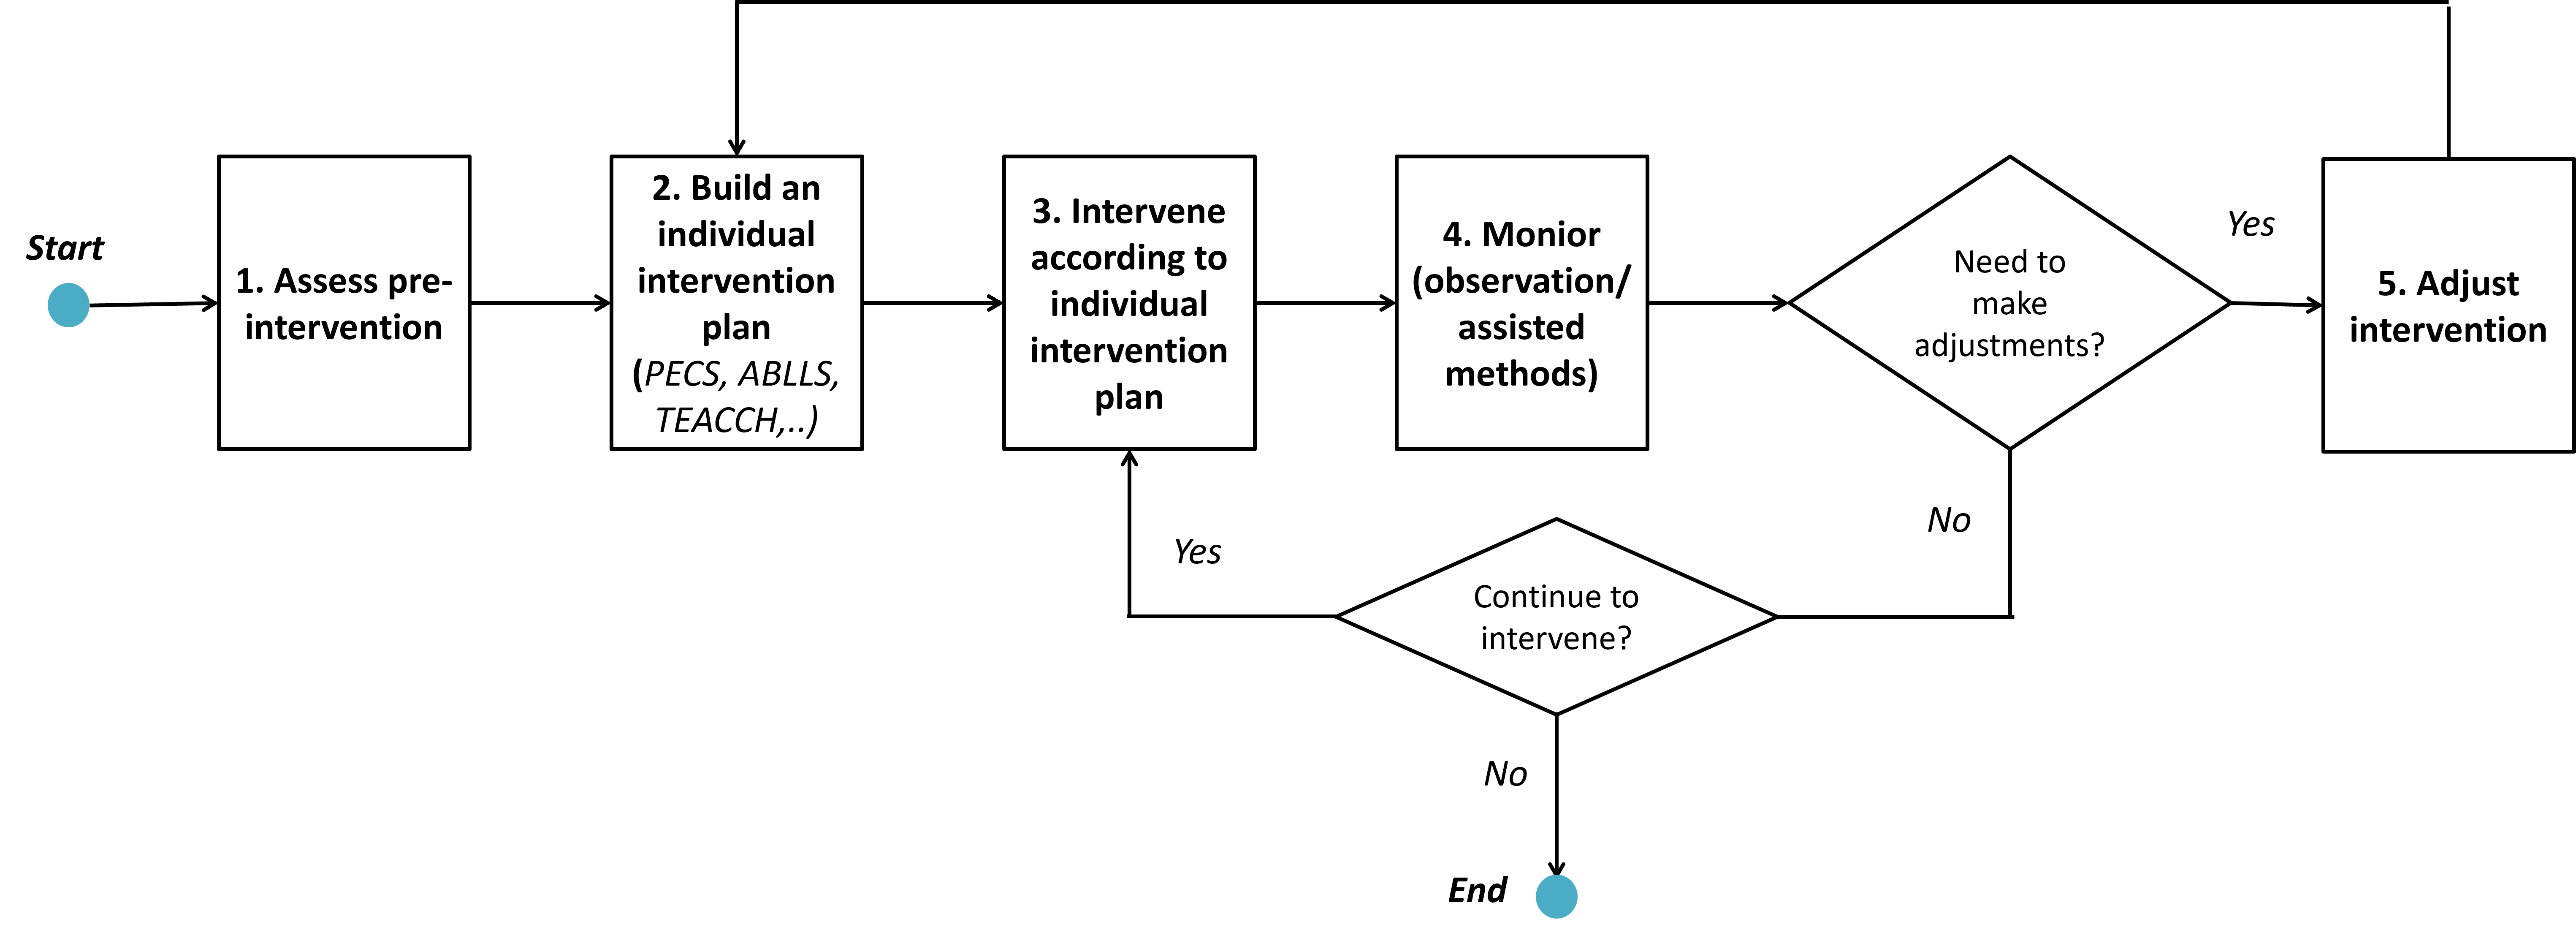
\includegraphics[width=1\columnwidth, alt={}]{samples/Data/fig1a.png}
    \caption{The 5 phases of the intervention cycle}
    \label{fig1}
\end{figure}

The landscape of intervention for children with ASD is characterized by a diverse array of methodologies, ranging from established traditional practices to newly validated scientific approaches. The scientific community generally concurs that no single method serves as a "cure-all" or is universally suitable for every child \cite{ref15,ref16}, a consensus that has driven a shift toward combined intervention strategies. Currently, psychological-educational intervention remains the dominant paradigm. This approach is grounded in the core principle of "compensation," which seeks to leverage a child’s inherent strengths to mitigate their weaknesses \cite{ref15}. Given that visual perception is frequently a relative strength for children with ASD \cite{ref18}, methodologies such as ABA, ABLLS-R, and the PECS have been widely adopted. PECS, for instance, exploits images and symbols to facilitate a stable and consistent mode of communication, effectively circumventing the transient and often confusing nature of spoken language \cite{ref19}.

To organize these disparate methods effectively, researchers have proposed a systematic, evidence-based meta-process known as the "guided intervention cycle" \cite{str01,str05}. As illustrated in figure \ref{fig1}, this process operates through five distinct phases: Assessment, where a profile of strengths and learning styles is developed; Planning, which involves creating measurable goals using frameworks like PECS or ABLLS; Implementation, the execution of the plan using evidence-based techniques; Monitoring, the collection of progress data; and Adjustment, where data is analyzed to modify strategies. Despite the theoretical robustness of this cycle, research indicates that the "Adjustment" phase represents a critical failure point \cite{str05,str04}. Current assessment practices are highly subjective, relying heavily on personal observation which creates susceptibility to bias. A failure at this stage effectively collapses the cycle's "early warning system," forcing practitioners into a reactive model where issues are addressed only after they have become severe.

\subsection{Information technology support (Robotics and VR)}
The inherent challenges and subjectivity of traditional observation have necessitated the development of information technology support methods. Prominent applications in this domain include socially assistive robots (SARs) \cite{new51} and virtual reality (VR) \cite{new52}. SARs are utilized as predictable social partners that help reduce anxiety, while VR offers controlled environments for social skill acquisition, ranging from immersive VR for high-functioning individuals to non-immersive setups for basic skill training. Additionally, mobile and wearable technologies have been introduced to facilitate physiological monitoring and real-time social coaching \cite{new56}

However, these technological interventions are not without significant limitations. The most critical drawback is the "generalization gap," wherein social skills acquired within controlled digital environments fail to transfer effectively to unpredictable, real-world scenarios. Furthermore, these automated interventions frequently lack the flexibility inherent in human therapy and often suffer from a paucity of long-term efficacy data, with many studies demonstrating only short-term improvements.

\subsection{Eye-tracking in ASD intervention}
ET technology has emerged as a potent tool to bridge the gap between subjective observation and objective data. Currently, ET is applied through two primary modalities: direct intervention and adaptive assessment. In direct intervention, systems such as Lookware™ \cite{ref11} integrate gaze-contingent ET (GCET) with ABA principles to provide immediate reinforcement when children focus on target facial areas, resulting in significant improvements in emotion recognition. regarding assessment, studies have utilized ET to tailor interventions to specific needs; for example, Giuliani \cite{ref09} utilized visual scanpaths to identify specific processing difficulties in adolescents, subsequently adapting the ABLLS-R program to address these deficits.

Despite this promise, current ET applications exhibit notable disadvantages within the "monitor" and "adjust" phases of the intervention cycle. Most existing systems monitor gaze in isolation, ignoring wider behavioral cues such as speech or motor responses that are visible to human experts. Moreover, raw ET data often lacks interpretability; while a system may detect that a child has averted their gaze, it cannot determine the underlying cause, such as fatigue versus disinterest. Consequently, automated adjustments are often restricted to rudimentary parameter changes, such as image brightness, rather than the complex clinical reasoning required for effective therapeutic modification.

\textbf{Summary}

In conclusion, while the field possesses a strong theoretical framework in the guided intervention cycle, practical application is hindered by the subjective nature of the "adjustment" phase. There is a distinct lack of tools capable of translating objective physiological data, such as ET metrics, into actionable, clinically relevant insights. This study aims to address this deficiency by developing a framework that empowers professionals to make data-driven decisions, thereby narrowing the division between theoretical potential and practical intervention utility.


\section{Methodology: Proposed eye-tracking framework}
\begin{figure}
    \centering
    
\includegraphics[width=1\columnwidth, alt={}]{samples/Data/fig1.png}
    \caption{Proposed integrated approach and system utility}
    \label{fig2}
\end{figure}





\subsection{Overview of the proposed method}

Interventions for children with ASD are traditionally structured within a sequential five-phase cycle. Within this lifecycle, the fourth phase of monitoring and evaluation is paramount for assessing behavioral responses and therapeutic efficacy. However, conventional monitoring relies heavily on subjective manual observation, a method prone to significant inter-rater variability which fundamentally compromises data fidelity.

To address these limitations, we introduce a quantitative framework that integrates ET technology directly into the standard intervention lifecycle. The fundamental objective is to transform the intervention pathway from a linear, qualitative process into a closed-loop, quantitative system. Functionally, this framework replaces subjective assessment with high-resolution oculometric data, specifically fixation duration and saccade patterns, enabling the capture of behavioral cues often imperceptible to human observation. The framework is architected around three core processes illustrated in figure \ref{fig2}: (1) baseline clinical assessment \& protocol design, (2) synchronized real-time oculomotor data collection, and (3) multidimensional behavioral analysis \& optimization.

\subsection{The 1st process - The foundational clinical assessment and protocol design}

The initial phase involves a multi-modal assessment designed to construct a high-dimensional profile for each participant. Data derived from standardized instruments and caregiver reports are synthesized to quantify disorder severity and specific sensory preferences. This comprehensive profiling informs the individualized intervention plan (IIP), ensuring that therapeutic goals adhere to SMART criteria (specific, measurable, attainable, relevant, time-bound).

Unlike unstructured approaches, this planning phase aligns rigorously with formalized methodologies. For example, within PECS, goals progress linearly from simple exchanges to complex discrimination tasks. Similarly, in the ABLLS-R, goals are linked to specific thematic content, such as visual performance puzzles. The proposed framework demonstrates maximum efficacy in visual-discrimination tasks where gaze metrics serve as a reliable proxy for cognitive processing.

\subsection{The 2nd process - The oculomotor data translation for adaptive intervention design}

The entire monitoring process for phase 4 of the intervention cycle was carried out using the ET-based framework we proposed in this study. Three main tasks were performed: visual feature extraction, rule-based establishment, and adjustment of recommended interventions.

\textbf{Extract visual feature:}  Feature extraction was performed using a framework from another study of ours, \cite{newETSAM}. This framework can quantify visual attention in a natural, dynamic environment to extract visual biomarkers from high-resolution natural video data. Automatic detection of visual signals was achieved by integrating eye-tracking with the Seament Anything Model; the main frame's output was quantified visual features of the participants. Additionally, the framework in the \cite{newETSAM} study allowed direct annotation of events mentioned in the $<Step 2 - Translating eye movement data for adaptive intervention design>$ within the ET signal. These events are spatially mapped to predefined areas of interest (AOIs) to generate semantic metrics, such as dwell time and transition matrix. 

\textbf{Establish rule-based:} The RBS functions as an inference engine, mapping semantic metrics to distinct behavioral states. The development of this engine follows a five-phase engineering framework:
\begin{enumerate}
    \item \textbf{Construct operationalization:} Defining target behaviors (e.g., "joint attention") based on established ASD symptomatology.
    \item \textbf{Threshold quantification:} Utilizing the Delphi method to establish reliable quantitative cut-offs (inter-rater reliability $\kappa > 0.7$).
    \item \textbf{Feature vectorization:} Converting raw data into logical inputs (e.g., "Gaze on Distractor $>$ Threshold").
    \item \textbf{Logic development:} Defining state transitions using conditional logic. For example:
    $$\text{IF } (\text{Avg fixation on distractor} > t_{time}) \text{ THEN } \text{Classification} = \text{"Task disengagement"}$$
    \item \textbf{Validation:} rigorous consistency checks against expert panels to ensure clinical validity.
\end{enumerate}


 
\textbf{Provide recommended intervention adjustment)}

This component operates as a clinical decision support system. Methodologically, the generation of recommendations is defined as a mapping function $R = f(S)$, which transforms the classified behavioral state $S$ into a specific recommendation output $R$.Crucially, the system utilizes a human-in-the-loop architecture. It is not designed to automate the physical intervention but to validate clinical observations with biometric evidence. Table \ref{tbadd1} illustrates the operational logic across different therapeutic contexts.

\begin{table}
    \caption{Illustrated according to the five-stage technical framework in 2 cases: PECS and ABLLS-R}
    \label{tb12}
    \renewcommand{\arraystretch}{3}
    \centering
    \small
    \begin{tabular}{|c|c|c|}
        \hline
        {\parbox{2cm}{\centering\textbf{Feature}}} 
        & {\parbox{5cm}{\textbf{Case 1: PECS (Social Attention Deficits)}}}
        & {\parbox{5cm}{\textbf{Case 2: ABLLS-R (Cognitive Disengagement)}}}
        \\ \hline

        {\parbox{2cm}{\textbf{Input (Process 1)}}}
        & {\parbox{5cm}{Gaze frequency/duration on “Partner AOI” vs “Object AOI”.}}
        & {\parbox{5cm}{Gaze frequency/duration on “Distractor AOIs” outside the workspace.}}
        \\ \hline

        {\parbox{2cm}{\textbf{Logic (Process 2)}}} 
        & {\parbox{5cm}{IF (Partner AOI Dwell $<$ Cutoff) AND (External Glance $>$ Threshold) THEN Class = “Impaired Social Exchange”}}
        & {\parbox{5cm}{IF (Distraction Fixation $>$ Cutoff) OR (Task AOI Focus $<$ Threshold) THEN Class = “Disengaged Task”}}
        \\ \hline

        {\parbox{2cm}{\textbf{Output (Process 3)}}} 
        & {\parbox{5cm}{Alert: “RECOMMENDATION: Social reference goal unassigned. Initiate ‘Look’ prompt.”}}
        & {\parbox{5cm}{Alert: “RECOMMENDATION: Attention drift detected ([X]s). Suggest verbal redirection.”}}
        \\ \hline

        {\parbox{2cm}{\textbf{Clinical Implication}}}
        & {\parbox{5cm}{Enables preemptive intervention before the child fails the social exchange.}}
        & {\parbox{5cm}{Differentiates between momentary pauses and true cognitive drift.}}
        \\ \hline
    \end{tabular}
    \label{tbadd1}
\end{table}


\subsection{The 3rd process - The multidimensional behavioral analysis and intervention optimization}

The final phase operates asynchronously to refine protocols between sessions. By integrating quantitative metrics with topological models, such as heat maps and scan paths, the system generates a clinical decision support report.

For instance, the system might yield an insight such as: "Participant focused 15\% on target images versus 40\% on environmental noise (instructor's clothing)." This granular level of data facilitates precise "environmental engineering," effectively closing the feedback loop. Based on these insights, the workflow bifurcates into two paths:
\begin{itemize}
    \item \textbf{Path A (Maintenance):} The current protocol is continued if deviations are statistically insignificant.
    \item \textbf{Path B (Optimization):} If deficits are confirmed, the intervention optimization protocol is triggered. This recursively directs the workflow back to the planning phase to recalibrate the IIP, ensuring continuous adaptation to the child's evolving needs.
\end{itemize}






% \begin{figure}
%     \centering
%     
\includegraphics[width=1\columnwidth, alt={}]{samples/Data/fig3.png}
%     \caption{A process for developing a rule base for assessing the behavior of children with autism spectrum disorder (ASD) during structured intervention}
%     \label{fig3}
% \end{figure}



% % \begin{table}[h]
    \caption{Information transforms raw, continuous time series data into discrete, quantifiable features suitable for IF-THEN logic}
    \centering
    \begin{tabular}{|c|c|c|}
    \hline
         \textbf{Behavior Classification}& \textbf{Rule Set  } & \textbf{Relevance of}\\ 
         \textbf{Scientific (Output)} & \textbf{(IF-THEN Logic)} &  \textbf{intervention}\\ \hline
         \textbf{PECS:} Impaired  & \textbf{IF (Dwell time on partner's } & Failure to meet  \\ 
         Social Exchange & AOI) AND (Glance away & social attention\\
           & from AOI in seconds),  & criteria for \\
             & THEN Classify as Impaired  & for PECS stages. \\
               & Social Exchange .  &  \\
          \hline
          \textbf{Thematic Awareness:} & IF (RJA Latency in  & Compare ET data with \\
          \textbf{RJA Error} & milliseconds) AND & established  \\
          & AND (Eye Tracking), & clinical/developmental   \\
           & THEN Classify as & endpoints.   \\
            & as RJA Error . &  \\
          \hline
    \end{tabular}
    \label{tba}
\end{table}

% \begin{table}[h]
%     \caption{Information transforms raw, continuous time series data into discrete, quantifiable features suitable for IF-THEN logic}
%     \centering
%     \begin{tabular}{|c|c|c|}
%     \hline
%          \textbf{Behavior Classification}& \textbf{Rule Set  } & \textbf{Relevance of}\\ 
%          \textbf{Scientific (Output)} & \textbf{(IF-THEN Logic)} &  \textbf{intervention}\\ \hline
%          \textbf{PECS:} Impaired  & \textbf{IF (Dwell time on partner's } & Failure to meet  \\ 
%          Social Exchange & AOI) AND (Glance away & social attention\\
%            & from AOI in seconds),  & criteria for \\
%              & THEN Classify as Impaired  & for PECS stages. \\
%                & Social Exchange .  &  \\
%           \hline
%           \textbf{Thematic Awareness:} & IF (RJA Latency in  & Compare ET data with \\
%           \textbf{RJA Error} & milliseconds) AND & established  \\
%           & AND (Eye Tracking), & clinical/developmental   \\
%            & THEN Classify as & endpoints.   \\
%             & as RJA Error . &  \\
%           \hline
%     \end{tabular}
%     \label{tba}
% \end{table}



\section{Experiment}

\subsection{Ethics and participants}
This study was conducted under the approval of the research ethics committee of the Hanoi University of Education. Written informed consent was obtained from the parents or legal guardians of all participants prior to enrollment. Participants were recruited from three specialized education centers, subject to strict inclusion criteria: (1) a confirmed diagnosis of ASD using the ADOS-21 assessment; (2) the absence of severe physical or neurological comorbidities; and (3) the cognitive and motor ability to successfully complete a 9-point ET calibration. From an initial pool of six candidates, three male participants ($N=3$) were selected for the longitudinal study, following the exclusion of two candidates due to calibration failure and one withdrawal. Information of the three participants is summarized in table \ref{tb1}

% \nopagebreak
\begin{table}
    \caption{Participant characteristics}
    \centering
    \small
    \begin{tabular}{|c|c|c|m{7cm}|}
    \hline
        {\textbf{No.}} & {\textbf{Participant}} & {\textbf{Age}} &{\textbf{Language ability}}\\
        \hline
        1 & 1st & 6 & Can say single words and double words but some words are unclear.\\ \hline
        2 & 2nd & 6 & Can speak but is mainly moving from imitative to proactive.\\ \hline
        3 & 3rd & 7 & Pronunciation difficulties.\\ \hline
    \end{tabular}
    \label{tb1}
\end{table}
\nopagebreak


% \begin{figure}
%     \centering
%     
\includegraphics[width=1\columnwidth, alt={}]{samples/Data/Picture2.png}
%     \caption{Experimental procedure}
%     \label{fig4}
% \end{figure}

\nopagebreak

\begin{figure}
    \centering
    \begin{tabular}{cc}
        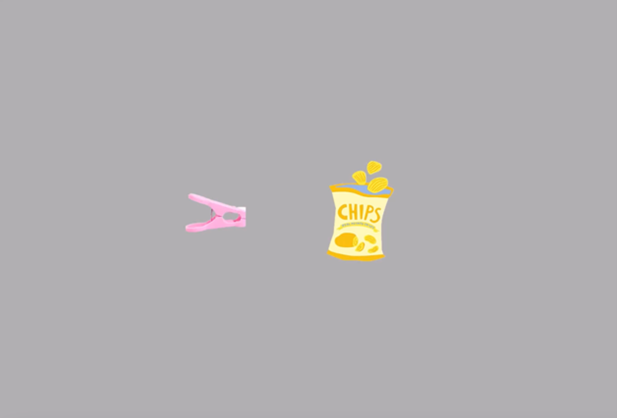
\includegraphics[width=6cm]{samples/Data/fig3a.png} &
        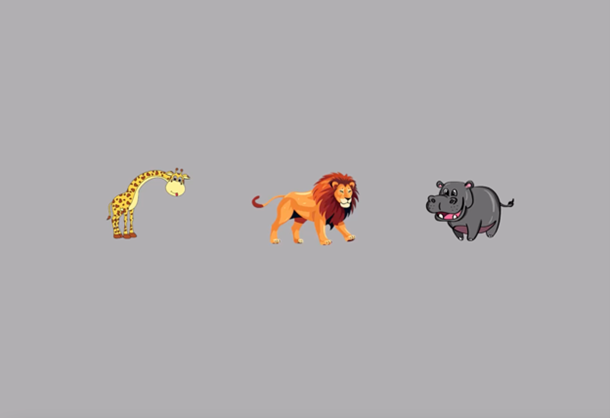
\includegraphics[width=6cm]{samples/Data/fig3b.png} \\
        (a) &
        (b)
    \end{tabular}
    \caption{Examples of stimuli used in the PECS phase 3 picture communication  intervention left (a) and ABLLS-R right(b)}
    \label{fig3}
\end{figure}
\nopagebreak



\subsection{Experimental design and stimuli}
The experiment utilized a multi-tiered stimulus design explicitly tailored to the cognitive profile and therapeutic stage of each child. Participant 1, currently in PECS phase 3, focused on object discrimination; stimuli were designed to juxtapose highly preferred items (e.g., favorite toys) against non-preferred items to elicit and measure selective gaze. Participant 2, engaging with the ABLLS-R thematic perception curriculum, focused on categorization tasks. Here, stimuli consisted of grids containing 4–6 semantically related objects (e.g., school supplies) to assess visual scanning efficiency. Figure \ref{fig3} illustrates the stimuli of participant 1 and participant 2 with two PECS phase 3 and ABLLS-R methods combined with thematic cognition, respectively. Participant 3, positioned in PECS phase 4, focused on sentence structure, utilizing complex multi-part visual frames (Subject + verb + object) to scaffold sentence construction. Figure \ref{fig4} illustrates the stimulus of participants in the three PECS phase 4 methods. To ensure the validity of these interventions, a consensus survey was conducted with domain experts ($N=31$) to establish a "ground truth" baseline regarding the expected intervention velocity for these specific tasks. Based on the visual stimuli designed to support the goals of each intervention, the eye-tracking metrics used to assess the effectiveness of the intervention goals for each child are listed in the table \ref{tb3}.

\begin{tableorg}
    \small
    \caption{Eye movement tracking indices for each participant}
    \label{tb3}
    \centering
    \renewcommand{\arraystretch}{1.7}
    \resizebox{\textwidth}{!}{
    \begin{tabular}{|c|c|c|c|}
    \hline
    \textbf{No.} & \textbf{Young} & \textbf{Intervention} & \parbox{7cm}{\centering \textbf{Eye tracking index}} \\ 
    \hline
    
    \multirow{6}{*}{1} 
    & \multirow{6}{*}{Subject 1} 
    & \multirow{6}{*}{PECS Phase 3 Communication}
    & Fixed number of times \\ \cline{4-4}
    & & & First fix \\ \cline{4-4}
    & & & Total fixed duration \\ \cline{4-4}
    & & & Ratio of fixed time to total observation time \\ \cline{4-4}
    & & & Number of discovered objects \\ \cline{4-4}
    & & & Percentage of time spent exploring each object \\ 
    \hline
    
    \multirow{6}{*}{2} 
    & \multirow{6}{*}{Subject 2} 
    & \multirow{6}{*}{Thematic awareness}
    & Total fixed duration \\ \cline{4-4}
    & & & Ratio of fixed time to total observation time \\ \cline{4-4}
    & & & Average Fixation Duration \\ \cline{4-4}
    & & & Fixed number of times \\ \cline{4-4}
    & & & Number of times the question was answered correctly \\ \cline{4-4}
    & & & Percentage of correct gaze when answering questions \\ 
    \hline
    
    \multirow{5}{*}{3} 
    & \multirow{5}{*}{Subject 3} 
    & \multirow{5}{*}{PECS Phase 4 Communication}
    & Total fixed duration \\ \cline{4-4}
    & & & Ratio of fixed time to total observation time \\ \cline{4-4}
    & & & Average Fixation Duration \\ \cline{4-4}
    & & & Fixed number of times \\ \cline{4-4}
    & & & View trajectory \\ 
    \hline
    \end{tabular}
        }
\end{tableorg}

\begin{figure}
    \centering
    \begin{tabular}{cc}
        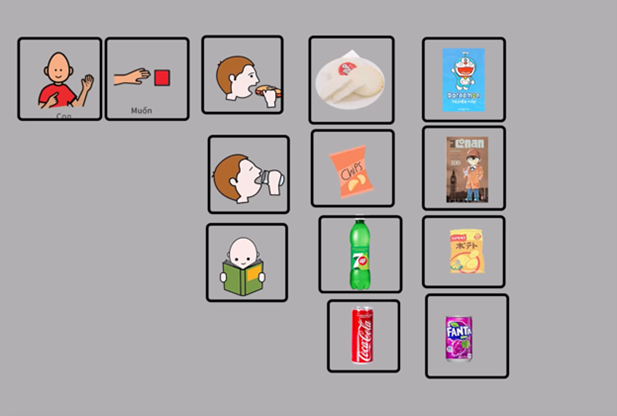
\includegraphics[width=6cm]{samples/Data/fig4a.png} &
        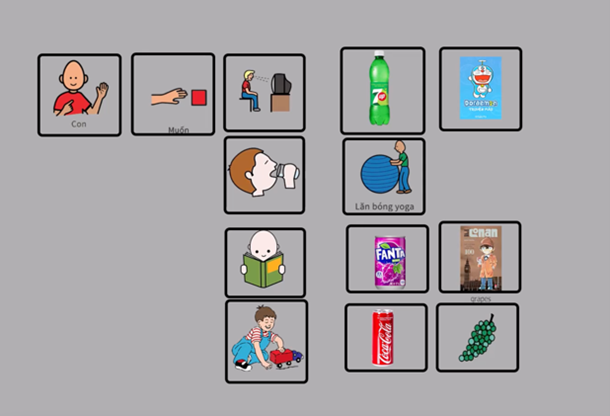
\includegraphics[width=6cm]{samples/Data/fig4b.png} \\
        (a) &
        (b)
    \end{tabular}
    \caption{Example of stimuli used in PECS phase 4 picture communication intervention}
    \label{fig4}
\end{figure}


\subsection{Experimental timeline (Longitudinal study)}
The study followed a four-phase longitudinal structure spanning approximately 3 months:
\begin{itemize}
    \item \textbf{Phase I - Baseline Characterization (Time 1):}
Prior to the commencement of the intervention, participants underwent standardized assessments (WISC-IV, ADI-R) alongside baseline ET sessions to establish initial cognitive and oculomotor profiles.
    \item \textbf{Phase II - Adaptive Intervention Loop (time 2 \& time 3):} This primary phase spanned two months and was bisected into two distinct cycles. Cycle 1 (Standard) involved the implementation of the initial IIP. Cycle 2 (Optimized) involved the recalibration of the intervention based on the RBS analysis of cycle 1 data. For instance, if the system detected a "left-side gaze bias," stimuli were strategically repositioned to accommodate or challenge this tendency.
    \item \textbf{Phase III - (Time 4):} Immediately following the intervention, the protocols from Phase I were repeated to quantify the delta in performance metrics.
    \item \textbf{Phase IV - Maintenance (Follow-up):} Assessments were performed at weeks 3 and 6 post-intervention without the assistance of the ET support system to evaluate skill maintenance and the generalization of learned behaviors.	
\end{itemize}

\subsection{Rule-based interpretation logic}

The core of the experimental framework relied on a RBS designed to translate raw ET metrics into actionable clinical recommendations. Rather than relying on raw data points, the RBS applied specific heuristics to interpret gaze behavior in context. For example, specific fixation durations were correlated with cognitive engagement, while erratic saccadic patterns were flagged as potential indicators of disinterest or sensory overload. The specific behavioral heuristics and interpretation logic utilized in this experiment are summarized in table \ref{tbadd2}.

\newcolumntype{L}[1]{>{\raggedright\arraybackslash}p{#1}}

\begin{table*}
\centering
\caption{Behavioral heuristics and interpretation logic}
\renewcommand{\arraystretch}{1.25}
\setlength{\tabcolsep}{5pt}

\begin{tabular}{|L{2.2cm}|L{2.8cm}|L{3cm}|L{7.2cm}|}
\hline
\textbf{Dimension} &
\textbf{Metric} &
\textbf{Logic / condition} &
\textbf{Clinical interpretation and recommendation} \\
\hline

\multirow{3}{2.2cm}{\textbf{1. Global engagement}} 
& \multirow{3}{2.8cm}{\textbf{Gaze ratio (Screen vs Off-screen)}}
& \textbf{Increase} ($\uparrow$)
& \textbf{Improved attention:} Reassess reward schedule; increase reinforcement quality. \\ \cline{3-4}

& 
& \textbf{Stable / Low} ($\rightarrow$)
& \textbf{Stagnation:} Shorten task duration; check environment for external distractions. \\ \cline{3-4}

&
& \textbf{Below Threshold} ($< \theta$)
& \textbf{Disengagement:} Alert therapist to re-engage child manually. \\
\hline

\multirow{2}{2.2cm}{\textbf{2. Processing strategy}}
& \multirow{2}{2.8cm}{\textbf{Fixation count vs duration}}
& \textbf{High Count + Low Duration}
& \textbf{Hyper-scanning:} Indicates confusion or overload. Recommendation: break task into smaller steps or clarify cues. \\ \cline{3-4}

&
& \textbf{Low count + high duration}
& \textbf{Deep Processing:} Indicates efficiency. Recommendation: proceed to next difficulty level. \\
\hline

\multirow{2}{2.2cm}{\textbf{3. Selective Attention}} 
& \multirow{2}{2.8cm}{\textbf{Target vs Distractor Ratio}}
& \textbf{Target $\uparrow$ + Distractor $\downarrow$}
& \textbf{Successful inhibition:} Strong indicator of task success. Recommendation: maintain current contrast levels. \\ \cline{3-4}

&
& \textbf{Distractor $\uparrow$}
& \textbf{Over-selectivity:} Child is distracted. Recommendation: simplify visual field (TEACCH principle) and increase target salience. \\
\hline

\multirow{2}{2.2cm}{\textbf{4. Proficiency}} 
& \multirow{2}{2.8cm}{\textbf{Response time vs accuracy}}
& \textbf{High accuracy + low time}
& \textbf{Mastery / Fluency:} Skill is automated. Recommendation: introduce generalization tasks. \\ \cline{3-4}

&
& \textbf{High accuracy + high time}
& \textbf{Compliance:} Accurate but hesitant. Recommendation: focus on fluency drills. \\
\hline

\end{tabular}
\label{tbadd2}
\end{table*}

\subsection{Clinical decision support strategy}
Based on the analysis generated by the RBS, the system employed two distinct optimization strategies to guide the intervention:
\begin{enumerate}
    \item \textbf{Optimization (Accommodation):} This strategy involved placing stimuli within the child's preferred visual region (e.g., the left hemifield) to maximize immediate success, reduce frustration, and build confidence.
    \item \textbf{Expansion (Remediation):} This strategy involved deliberately placing stimuli outside the preferred region. This approach was utilized to challenge the participant, forcing them to expand their visual scanning field and actively overcome specific attentional deficits.
\end{enumerate}

\subsection{Data analysis and validation strategy}
To validate the clinical efficacy of the proposed framework, a comparative analysis was executed to contrast system-driven intervention outcomes against a baseline of expert consensus. To establish this "Ground truth" a survey was administered to a cohort of $N=31$ ASD professionals, comprising special education teachers and therapists. These experts reviewed the baseline clinical profiles of the three study participants and formulated predictive estimates regarding the temporal investment required and the anticipated level of achievement for each intervention goal under standard therapeutic conditions.


The core analytical metric was defined as the delta between these predicted outcomes (Expert consensus) and the actual outcomes achieved through the ET-assisted intervention. The data were evaluated based on three statistical criteria: immediacy (the latency of behavioral change), overlap (the consistency of performance across sessions), and trend direction. Within this experimental design, success was rigorously defined as the participant achieving the target goals with greater efficiency (reduced time-to-acquisition) or higher proficiency than the benchmarks established by the expert panel.


% \begin{sidewaystable*}
%     \small
%     \renewcommand{\arraystretch}{2}
%     \centering
    
 \begin{tableorg}
    \small
    \caption{Eye tracking index for all frames in 4 data acquisitions of participant 1}
    \renewcommand{\arraystretch}{2}
     \centering
     \resizebox{\textwidth}{!}{
    \begin{tabular}{|c|c|c|c|c|c|c|c|c|c|c|c|}
    \hline
          \multicolumn{2}{c|}{}  
          & \multicolumn{6}{c|}{\textbf{Frame}} 
          & \multirow{2}{*}{{\parbox{2cm}{\centering\textbf{Number of frames the child sees}}}} 
          & \multirow{2}{*}{{\parbox{2cm}{\centering\textbf{Total fixed duration (ms)}}}} 
          & \multirow{2}{*}{{\parbox{2cm}{\centering\textbf{Fixed number of times}}}} 
          & \multirow{2}{*}{\parbox{2cm}{\centering\textbf{Average fixed time}}} \\ \cline{3-8}
          \multicolumn{2}{c|}{} & 1 & 2 & 3 & 4 & 5 & 6 &  &  &  & \\ \hline
   
    \multirow{2}{*}{\textbf{First time}}
         & (1) & 0 & 1 & 1 & 0 & 1 & 0 & \multirow{2}{*}{3/6} & \multirow{2}{*}{1230} & \multirow{2}{*}{9} & \multirow{2}{*}{136.67} \\ \cline{2-8}
         & (2) & 0 & 367 & 401 & 0 & 462 & 0 &  &  &  &  \\ \hline
    \multirow{2}{*}{\textbf{2nd time} }
         & (1) & 0 & 1 & 1 & 1 & 1 & 0 & \multirow{2}{*}{4/6} & \multirow{2}{*}{54120} & \multirow{2}{*}{4} & \multirow{2}{*}{13530} \\ \cline{2-8}
         & (2) & 0 & 12969 & 13460 & 14725 & 12966 & 0 &  &  &  &  \\ \hline
    \multirow{2}{*}{\textbf{3rd time} }
         & (1) & 1 & 1 & 1 & 2 & 1 & 1 & \multirow{2}{*}{6/6} & \multirow{2}{*}{7276} & \multirow{2}{*}{34} & \multirow{2}{*}{214} \\ \cline{2-8}
         & (2) & 720 & 757 & 331 & 1568 & 2459 & 1441 &  &  &  &  \\ \hline
    \multirow{2}{*}{\textbf{4th time} }
         & (1) & 2 & 2 & 1 & 1 & 1 & 1 & \multirow{2}{*}{6/6} & \multirow{2}{*}{3046} & \multirow{2}{*}{20} & \multirow{2}{*}{152.3} \\ \cline{2-8}
         & (2) & 1532 & 468 & 336 & 108 & 131 & 471 &  &  &  &  \\ \hline
     \end{tabular}
        }
    \label{tb4}
    \vspace{2mm}
    \begin{flushleft}
    \footnotesize
    \textsuperscript{(1)} Number of young people exploring. \hspace{5mm}
    \textsuperscript{(2)} Fixed duration.
    \end{flushleft}
\end{tableorg}

% (1) Number of young people exploring
% (2) Fixed duration






\begin{sidewaystable*}
    \small
    \renewcommand{\arraystretch}{1.6}
    \centering
    \caption{Eye movement tracking index by location and object displayed throughout the entire stimulus video of participant 1}
    \centering
    \resizebox{\textwidth}{!}{
    \begin{tabular}{|c|c|c|c|c|c|c|c|p{3cm}|}
    \hline
        
        \multicolumn{2}{c|}{} & \multicolumn{4}{c|}{\textbf{Object of view}} & \multicolumn{2}{c|}{\textbf{Object display position}} & \\ \cline{3-8}
        
         \multicolumn{2}{c|}{\parbox{3cm}{\textbf{Number of appearances}}}  & \textbf{Car} & \textbf{Rice cake} & \textbf{Clip} & \textbf{Snacks} & \multirow{2}{*}{\textbf{Left}} & \multirow{2}{*}{\textbf{Right}} & \\ \cline{3-6}
         
         \multicolumn{2}{c|}{}  & 2 & 1 & 6 & 3 &  &  & \\ \hline
         
         \multirow{2}{*}{\textbf{First Time}}  
         & \textbf{(1)} & 2 & 1 & 0 & 0 & 2 & 1 
         & \multirow{8}{*}{\parbox{3cm}{\textbf{Number of objects the child looks at throughout the video}}} \\ \cline{2-8}
         & \textbf{(2)} & 66.67 & 33.33 & 0 & 0 & 66.67 & 33.33 & \\ \cline{1-8}
         
         \multirow{2}{*}{\textbf{2nd Time}}& \textbf{(1)} & 1 & 1 & 2 & 0 & 1 & 0 & \\ \cline{2-8}
         & \textbf{(2)} & 25 & 25 & 50 & 0 & 100 & 0 & \\ \cline{1-8}
         
         \multirow{2}{*}{\textbf{3rd Time}}& \textbf{(1)} & 2 & 1 & 1 & 4 & 3 & 5 & \\ \cline{2-8}
         & \textbf{(2)} & 25 & 12.5 & 12.5 & 50 & 37.5 & 62.5 & \\ \cline{1-8}
         
         \multirow{2}{*}{\textbf{4th Time}}& \textbf{(1)} & 2 & 1 & 2 & 3 & 4 & 4 & \\ \cline{2-8}
         & \textbf{(2)} & 25 & 12.5 & 25 & 37.5 & 50 & 50 & \\ \hline
         
         
         \multirow{2}{*}{\textbf{First Time}}& \textbf{(3)} & 6 & 3 & 0 & 0 & 6 & 3 & \multirow{8}{*}{\parbox{3cm}{\textbf{Fixed number of times for each object}}}\\ \cline{2-8}
         & \textbf{(2)} & 66.67 & 33.33 & 0 & 0 & 66.67 & 33.33 & \\ \cline{1-8}
         
         \multirow{2}{*}{\textbf{2nd Time}} & \textbf{(3)} & 1 & 1 & 2 & 0 & 8 & 0 & \\ \cline{2-8}
         & \textbf{(2)} & 25 & 25 & 50 & 0 & 100 & 0 & \\ \cline{1-8}
         
         \multirow{2}{*}{\textbf{3rd Time}}& \textbf{(3)} & 13 & 3 & 1 & 17 & 26 & 42 & \\ \cline{2-8}
         & \textbf{(2)} & 38.24 & 8.82 & 2.94 & 50 & 38.24 & 61.76 & \\  \cline{1-8}
         
         \multirow{2}{*}{\textbf{4th Time}}& \textbf{(3)} & 6 & 2 & 5 & 7 & 18 & 22 & \\  \cline{2-8}
         & \textbf{(2)} & 30 & 10 & 25 & 35 & 45 & 55 & \\  \hline
         
    %      \multirow{2}{*}{\textbf{First Time}}& \textbf{(4)} & 829 & 401 & 0 & 0 & 863 & 367 & \multirow{8}{*}{\parbox{3cm}{\textbf{Fixed duration for each subject}}}\\  \cline{2-8}
         
    %      & \textbf{(2)} & 67.4 & 32.6 & 0 & 0 & 70.16 & 29.84 & \\  \cline{1-8}
    %      \multirow{2}{*}{\textbf{2nd Time}}& \textbf{(4)} & 12966 & 13460 & 27694 & 0 & 54120 & 0 & \\  \cline{2-8}
    %      & \textbf{(2)} & 23.96 & 24.87 & 51.17 & 0 & 100 & 0 & \\  \cline{1-8}
    %      \multirow{2}{*}{\textbf{3rd Time}}& \textbf{(4)} & 3216 & 331 & 144 & 3585 & 2934 & 4342 & \\  \cline{2-8}
    %      & \textbf{(2)} & 44.20 & 4.55 & 1.98 & 49.27 & 40.32 & 59.68 & \\  \cline{1-8}
    %      \multirow{2}{*}{\textbf{4th Time}} & \textbf{(4)} & 447 & 336 & 1066 & 1197 & 1533 & 1513 & \\  \cline{2-8}
    %      & \textbf{(2)} & 14.68 & 11.02 & 35 & 39.3 & 50.33 & 49.67 & \\ \hline
    \end{tabular}
        }
    \label{tb5}

    
\end{sidewaystable*}

\begin{sidewaystable*}
    \small
    \renewcommand{\arraystretch}{1.6}
    % \centering
    \resizebox{\textwidth}{!}{
    \begin{tabular}{|c|c|c|c|c|c|c|c|p{3cm}|}
    \hline
        
        \multicolumn{2}{c|}{} & \multicolumn{4}{c|}{\textbf{Object of view}} & \multicolumn{2}{c|}{\textbf{Object display position}} & \\ \cline{3-8}
        
         \multicolumn{2}{c|}{\parbox{3cm}{\textbf{Number of appearances}}}  & \textbf{Car} & \textbf{Rice cake} & \textbf{Clip} & \textbf{Snacks} & \multirow{2}{*}{\textbf{Left}} & \multirow{2}{*}{\textbf{Right}} & \\ \cline{3-6}
         
         \multicolumn{2}{c|}{}  & 2 & 1 & 6 & 3 &  &  & \\ \hline      
                  
         \multirow{2}{*}{\textbf{First Time}}& \textbf{(4)} & 829 & 401 & 0 & 0 & 863 & 367 & \multirow{8}{*}{\parbox{3cm}{\textbf{Fixed duration for each subject}}}\\  \cline{2-8}
         
         & \textbf{(2)} & 67.4 & 32.6 & 0 & 0 & 70.16 & 29.84 & \\  \cline{1-8}
         \multirow{2}{*}{\textbf{2nd Time}}& \textbf{(4)} & 12966 & 13460 & 27694 & 0 & 54120 & 0 & \\  \cline{2-8}
         & \textbf{(2)} & 23.96 & 24.87 & 51.17 & 0 & 100 & 0 & \\  \cline{1-8}
         \multirow{2}{*}{\textbf{3rd Time}}& \textbf{(4)} & 3216 & 331 & 144 & 3585 & 2934 & 4342 & \\  \cline{2-8}
         & \textbf{(2)} & 44.20 & 4.55 & 1.98 & 49.27 & 40.32 & 59.68 & \\  \cline{1-8}
         \multirow{2}{*}{\textbf{4th Time}} & \textbf{(4)} & 447 & 336 & 1066 & 1197 & 1533 & 1513 & \\  \cline{2-8}
         & \textbf{(2)} & 14.68 & 11.02 & 35 & 39.3 & 50.33 & 49.67 & \\ \hline
    \end{tabular}
        }
    \label{tb5}
    
    \vspace{2mm}
    \begin{flushleft}
    \footnotesize
    \textsuperscript{(1)} Number of views. \hspace{5mm}
    \textsuperscript{(2)} Ratio. \hspace{5mm}
    \textsuperscript{(3)} Fixed number of times. \hspace{5mm}
    \textsuperscript{(4)} Fixed duration. \hspace{5mm}
    \end{flushleft}
    
\end{sidewaystable*}

% (1) Number of views
% (2) Ratio
% (3) Fixed number of times
% (4) Fixed duration


\section{Results}
\subsection{Participant 1: Mitigating lateral bias (PECS phase 3)}
Objective: Object discrimination (Preferred vs. non-preferred).

Eye-tracking indices for all frames across 4 data acquisitions, and by location and object displayed throughout the entire stimulus video of participant 2, are presented in the table \ref{tb4}, \ref{tb5}.



\subsubsection{Baseline analysis (Time 1):} Figure \ref{fig11} presents the eye movement tracking metrics of the first participant over four recordings. Initial oculometric analysis revealed a severe deficit in visual coverage. The participant explored only 3 out of the 6 available frames, exhibiting a notably short average fixation duration of 136.67 ms. Crucially, the generated heat maps exposed a pronounced Left-Side Lateral bias, with $66.67\%$ of fixation points concentrated exclusively on the left hemifield. This asymmetry caused the child to systematically ignore objects placed on the right, resulting in successful attention to only 2 out of 4 target objects.

\begin{figure}
    \centering
    \begin{tabular}{ccc}
        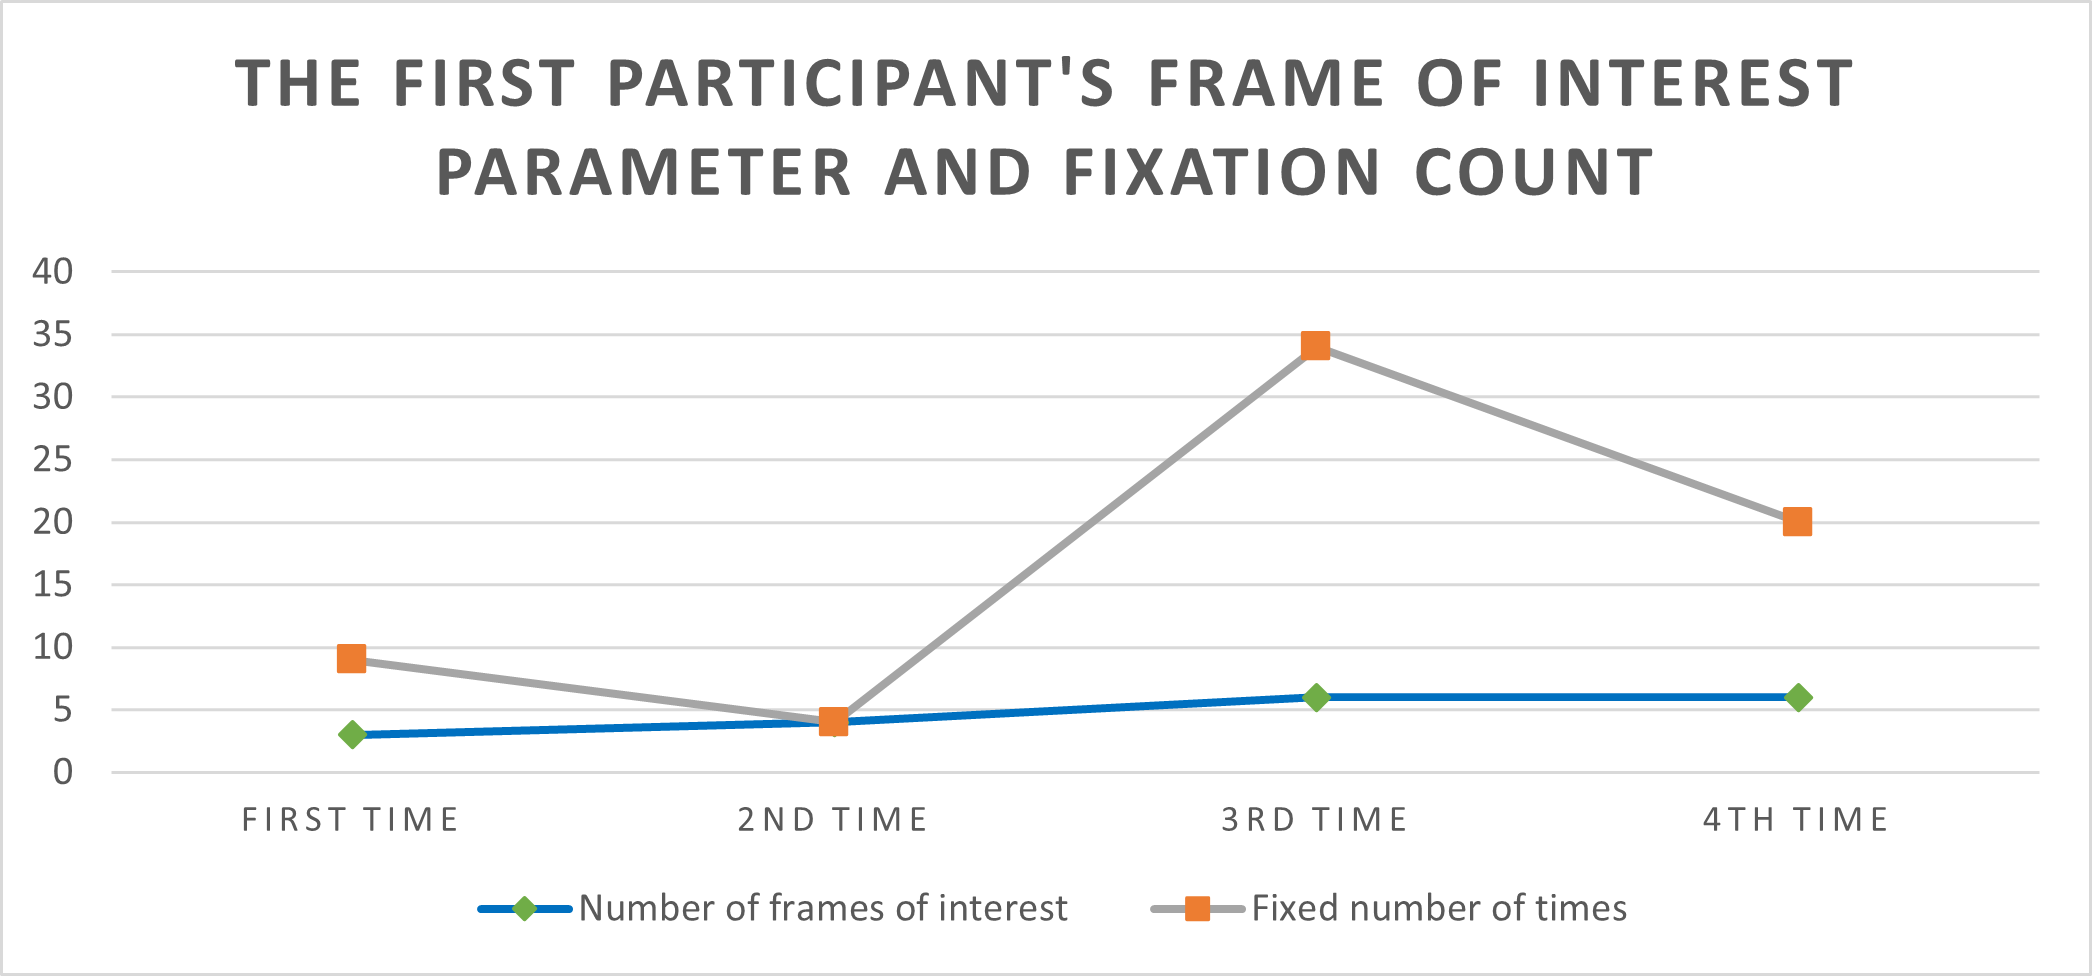
\includegraphics[width=4.1cm]{samples/Data/fig10a.png} &
        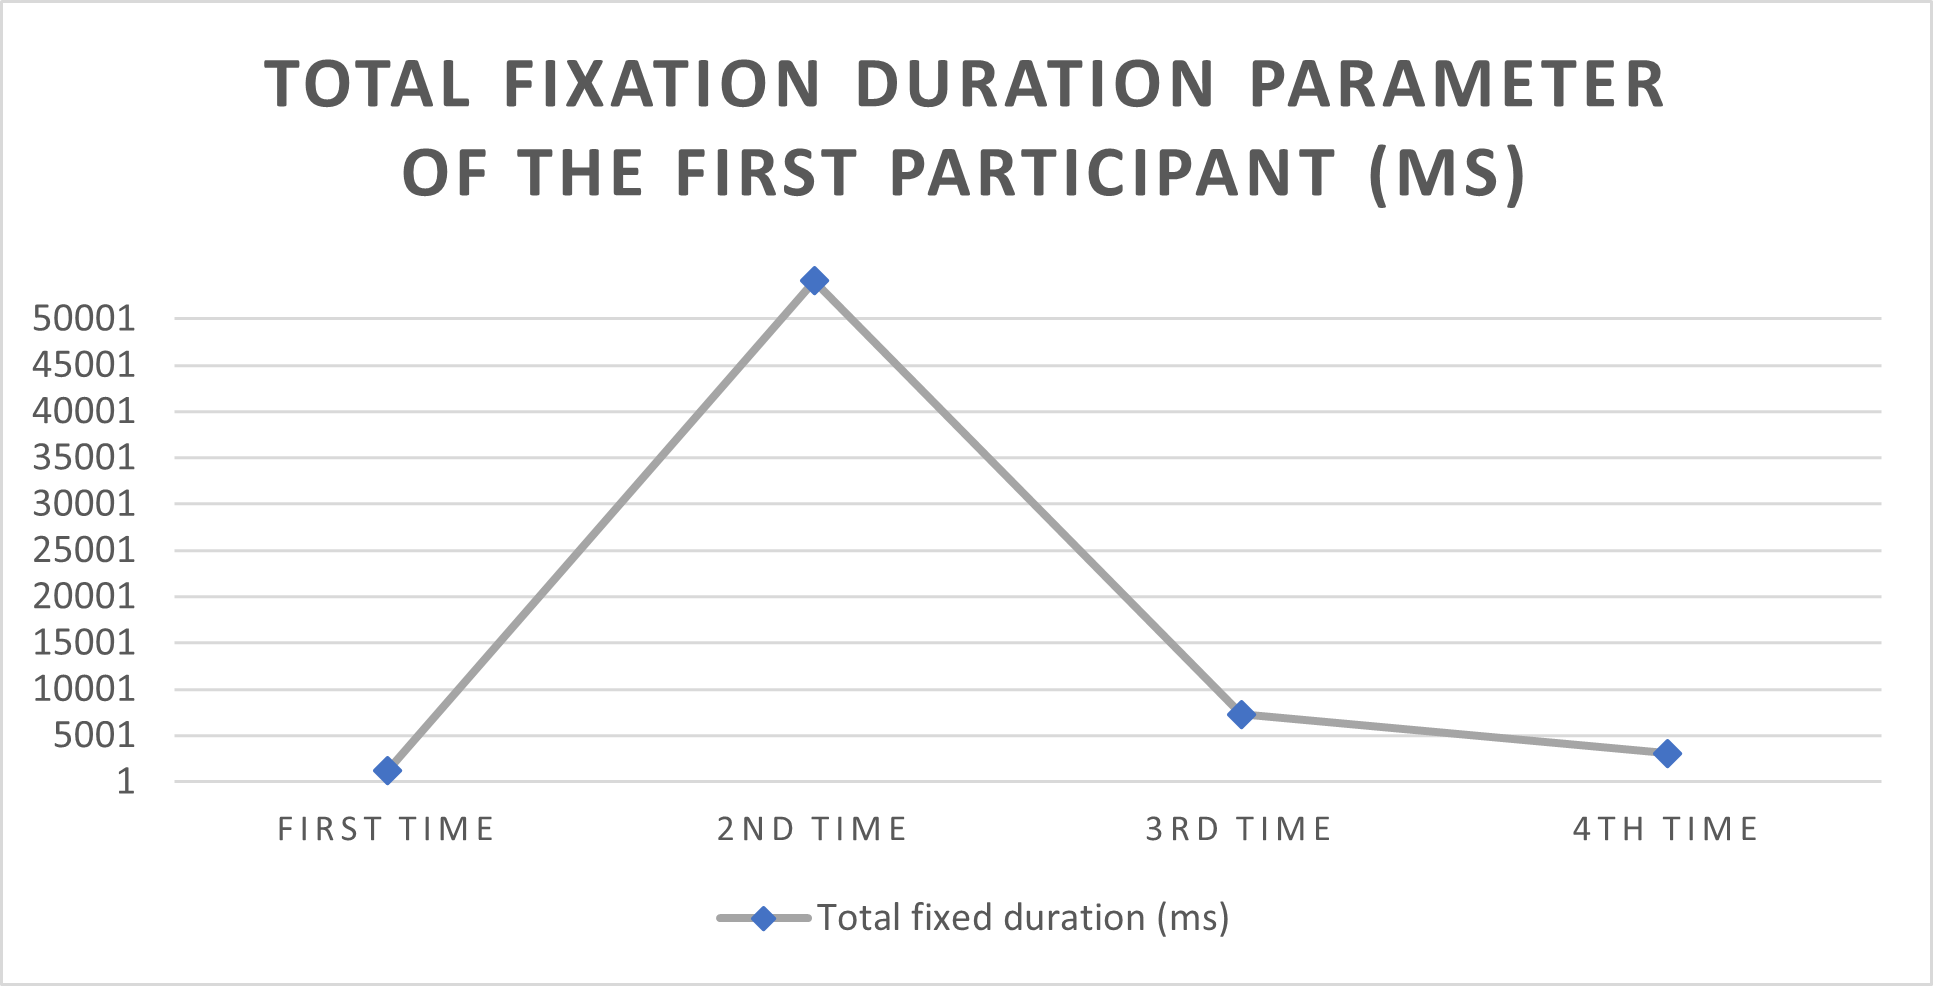
\includegraphics[width=4.1cm]{samples/Data/fig10b.png}&
        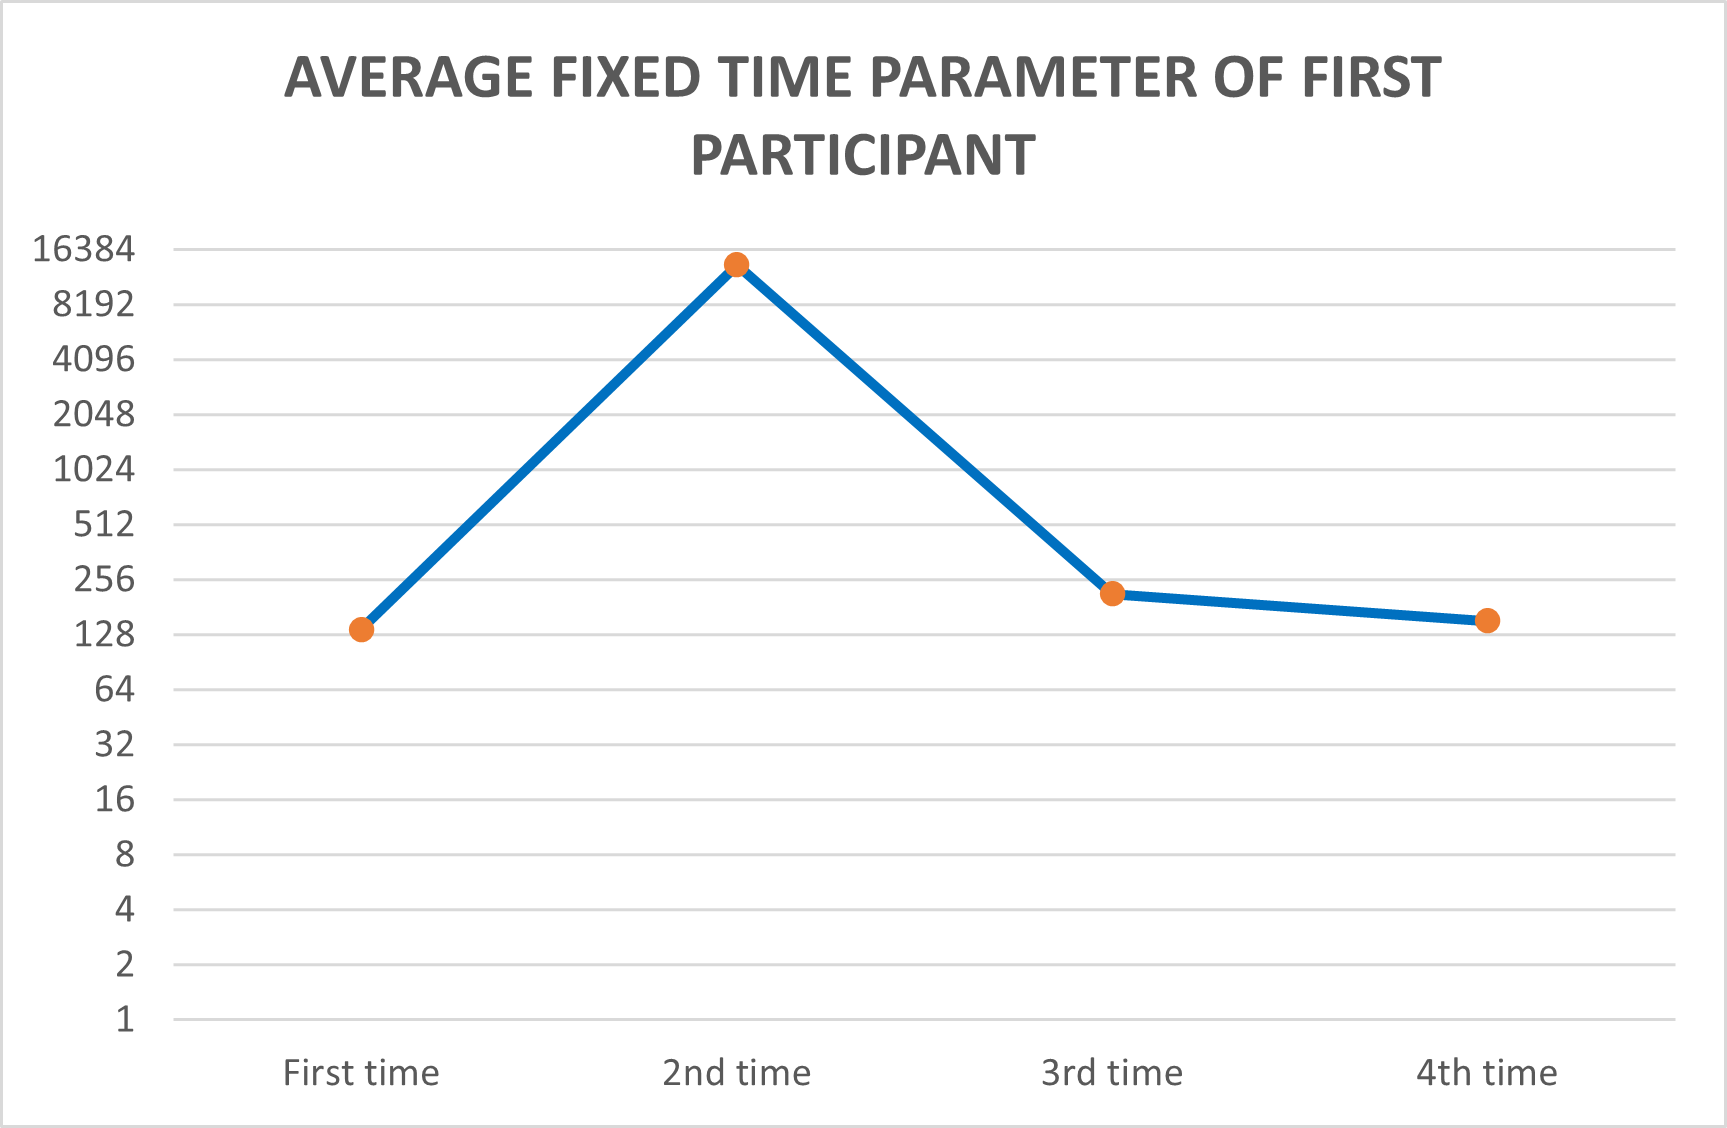
\includegraphics[width=4cm]{samples/Data/fig10c.png}\\
        (a) &
        (b)&
        (c)
    \end{tabular}
    \caption{Compare the parameters of the first participant explores on the number of frames and the number of fixes (a);total fixed duration (b); and average fixed time (c) in each phase}
    \label{fig11}
\end{figure}

\subsubsection{Cycle 1: Optimization (Accommodation strategy):} Based on the "left-side bias" detected by the RBS, the intervention was initially adjusted to accommodate this sensory preference. Visual aids and novel concepts were strategically positioned within the left and center fields of view to maximize engagement. Assessment at time 2 demonstrated a marked improvement in engagement, with the participant exploring 4 out of 6 frames. However, the system flagged a critical secondary risk: fixation intensity on the left side rose to $100\%$, indicating the potential development of a stereotypical gaze pattern rather than flexible attention.

\subsubsection{Cycle 2: Remediation (Expansion strategy):} To mitigate the risk of entrenched stereotype, the RBS triggered the Expansion Protocol. During review activities, stimuli were gradually shifted from the left to the right field to force active visual scanning. This adjustment proved highly effective at time 3, with the participant successfully exploring 6 out of 6 frames ($100\%$ coverage). Most significantly, the lateral bias was neutralized; $62.5\%$ of fixations shifted to the correct position on the right side, confirming that the child had successfully broken the fixed gaze habit. Figure \ref{fig9} shows a heatmap illustration of a baseline frame, which shows a relatively narrow field of view, with most of the gaze focused to the left. However, at cycle two interaction time, the child's field of view has expanded and gradually shifted to the right.



\begin{figure}
    \centering
    \begin{tabular}{cc}
        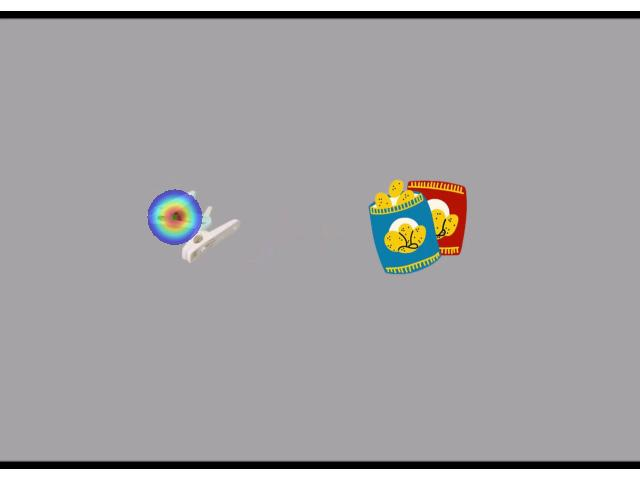
\includegraphics[width=6.5cm]{samples/Data/fig8a.jpg} &
        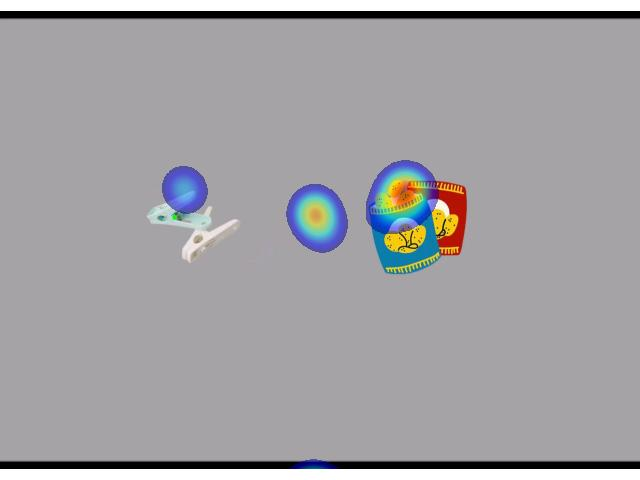
\includegraphics[width=6.5cm]{samples/Data/fig8b.jpg} \\
        (a) &
        (b)
    \end{tabular}
    \caption{Heatmap of a frame at (a) the baseline and (b) after cycle 2 intervention times of the 1st participant}
    \label{fig9}
\end{figure}
    







\subsubsection{Maintenance (Time 4):} Follow-up assessments conducted without ET support indicated sustained skill acquisition. Frame exploration remained maximal, and fixation durations stabilized, suggesting that the expanded visual range had been internalized as a functional behavioral trait.

\subsection{Participant 2: Enhancing Thematic Perception (ABLLS-R)}
Objective: Categorization and Identification.

Eye-tracking indices for all frames across 4 data acquisitions, and by location and object displayed throughout the entire stimulus video of participant 2, are presented in the table \ref{tb6}, \ref{tb7}.



 \begin{tableorg}
    \small
    \caption{Eye tracking index for all frames in 4 data acquisitions of participant 2}
    \renewcommand{\arraystretch}{2}
    \centering
    \resizebox{\textwidth}{!}{
    \begin{tabular}{|c|c|c|c|c|c|c|c|c|c|c|c|c|}
    \hline
         \multicolumn{2}{c|}{}& \multicolumn{6}{c|}{\textbf{Frame}} &  \multirow{2}{*}{\parbox{2cm}{\textbf{Correct answer rate}}} & \multirow{2}{*}{\parbox{2cm}{\textbf{Number of frames the child sees}}} & \multirow{2}{*}{\parbox{2cm}{\textbf{Total fixed duration (ms)}}} & \multirow{2}{*}{\parbox{2cm}{\textbf{Fixed number of times}}} & \multirow{2}{*}{\parbox{2cm}{\textbf{Average fixed time}}}\\ \cline{3-8}
         \multicolumn{2}{c|}{} & 1 & 2 & 3 & 4 & 5 & 6 &  &  &  &  & \\ \hline
         \multirow{2}{*}{\textbf{First Time}}& \textbf{(1)} & 0 & 0 & 0 & 0 & 0 & 1 & \multirow{2}{*}{0/6} & \multirow{2}{*}{1/6} & \multirow{2}{*}{5321} & \multirow{2}{*}{5} & \multirow{2}{*}{106.2}\\ \cline{2-8}
         & \textbf{(2)} & 0 & 0 & 0 & 0 & 0 & 531 &  &  &  &  & \\ \hline
         \multirow{2}{*}{\textbf{2nd Time}}& \textbf{(1)} & 0 & 2 & 1 & 1 & 1 & 1 & \multirow{2}{*}{2/6} & \multirow{2}{*}{5/6} & \multirow{2}{*}{1618} & \multirow{2}{*}{13} & \multirow{2}{*}{124.46}\\ \cline{2-8}
         & \textbf{(2)} & 0 & 470 & 57 & 301 & 524 & 266 &  &  &  &  & \\ \hline
         \multirow{2}{*}{\textbf{3rd Time}}& \textbf{(1)} & 1 & 1 & 2 & 1 & 3 & 0 & \multirow{2}{*}{4/6} & \multirow{2}{*}{5/6} & \multirow{2}{*}{8245} & \multirow{2}{*}{45} & \multirow{2}{*}{183.22}\\  \cline{2-8}
         & \textbf{(2)} & 2201 & 236 & 2081 & 444 & 3283 & 0 &  &  &  &  & \\ \hline
         \multirow{2}{*}{\textbf{4th Time}}& \textbf{(1)} & 2 & 3 & 2 & 2 & 1 & 1 & \multirow{2}{*}{6/7} & \multirow{2}{*}{6/6} & \multirow{2}{*}{3491} & \multirow{2}{*}{28} & \multirow{2}{*}{124.68}\\  \cline{2-8}
         & \textbf{(2)} & 687 & 563 & 558 & 214 & 518 & 951 &  &  &  &  & \\ \hline
     \end{tabular}
        }
    \label{tb6}
    \vspace{2mm}
    \begin{flushleft}
    \footnotesize
    \textsuperscript{(1)} Number of young people exploring. \hspace{5mm}
    \textsuperscript{(2)} Fixed duration.
    \end{flushleft}
 \end{tableorg}

% (1) Number of young people exploring
% (2) Fixed duration

\input{tables/table_7}

\subsubsection{Baseline analysis (Time 1):} Figure \ref{fig14} presents the eye movement tracking metrics of the second participant over four recordings. Baseline metrics indicated extremely low cognitive engagement. The participant exhibited a pattern of "attentional tunneling," focusing exclusively on a single "favorite object" (a leopard) located in the center of the array while ignoring all other stimuli. This resulted in a $100\%$ fixation rate on the center object and a $0\%$ correct response rate. Furthermore, scan path analysis revealed a restriction to vertical scanning, with a complete absence of horizontal search behavior. Figure \ref{figcycle1} shows the vertical viewing tendency illustrated through the scanpath of the second participant.

\begin{figure}
    \centering
    \begin{tabular}{ccc}
        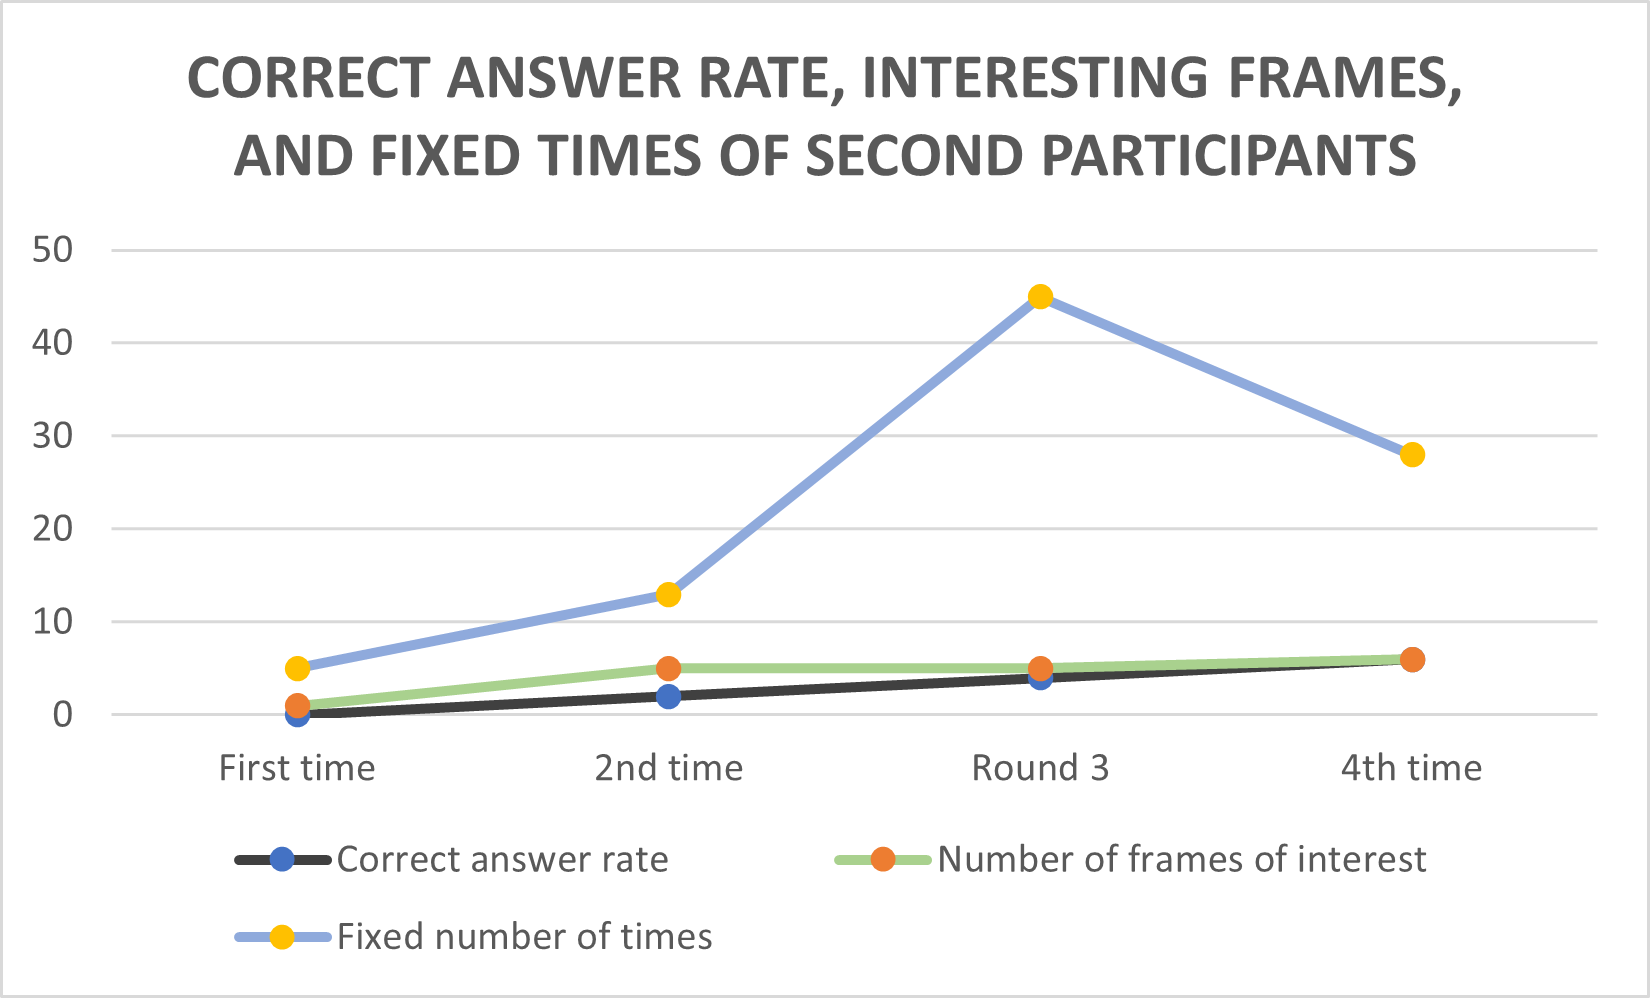
\includegraphics[width=4.1cm]{samples/Data/fig13a.png} &
        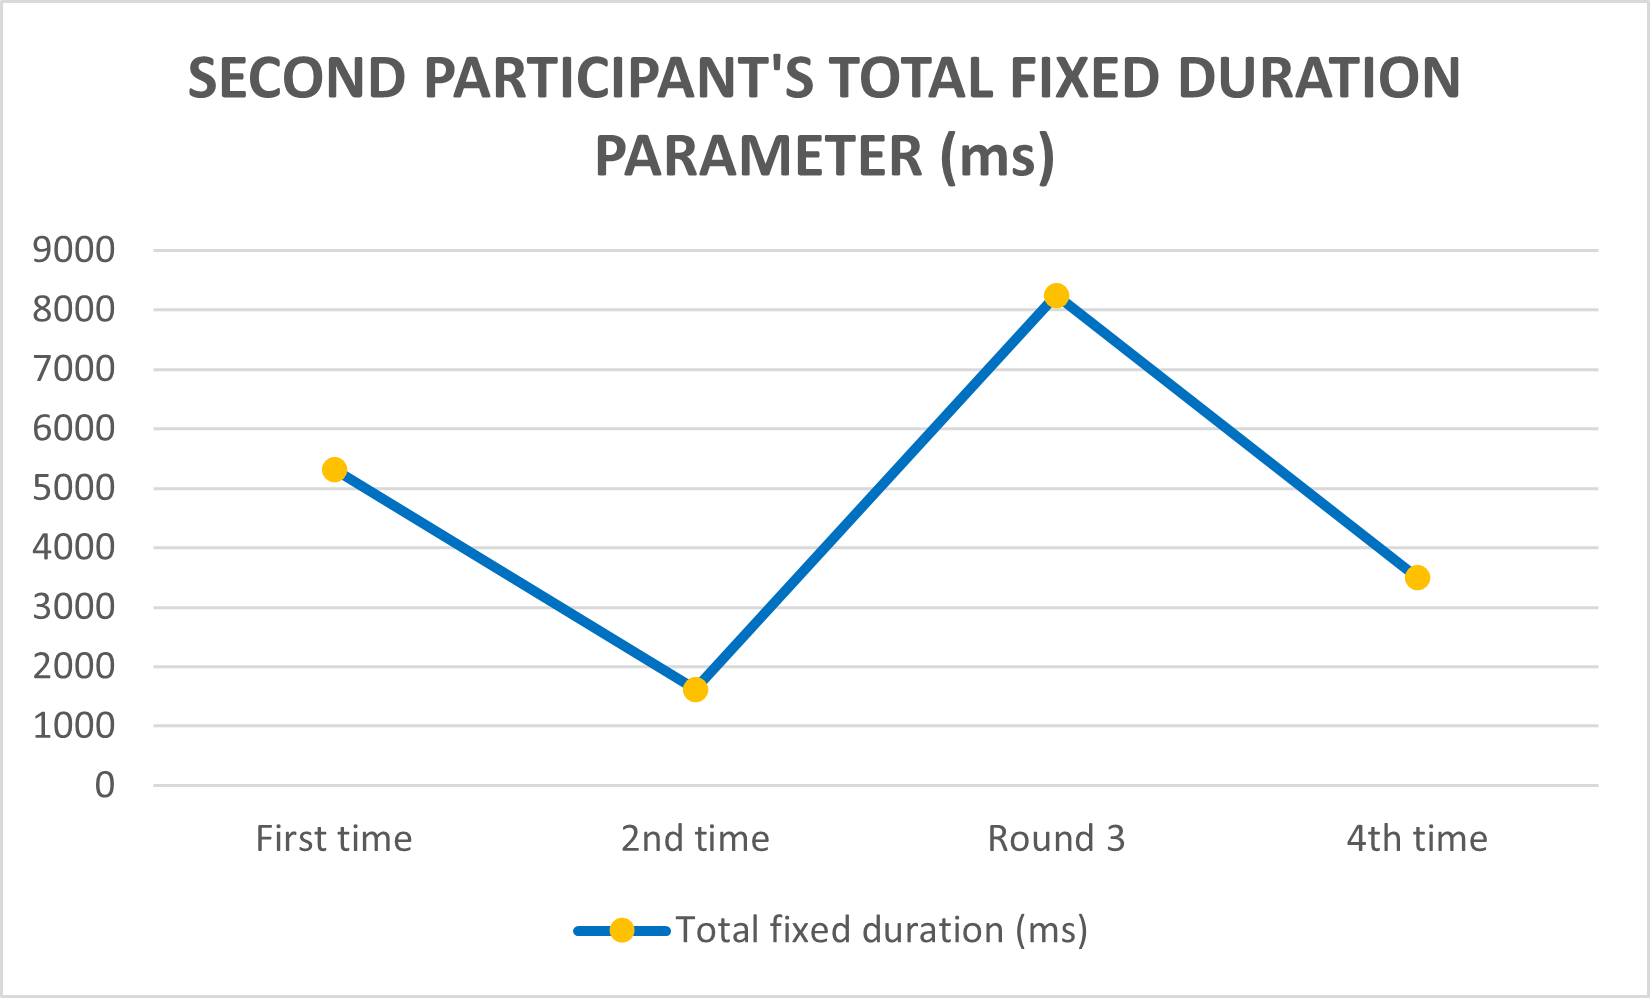
\includegraphics[width=4.1cm]{samples/Data/fig13b.png}&
        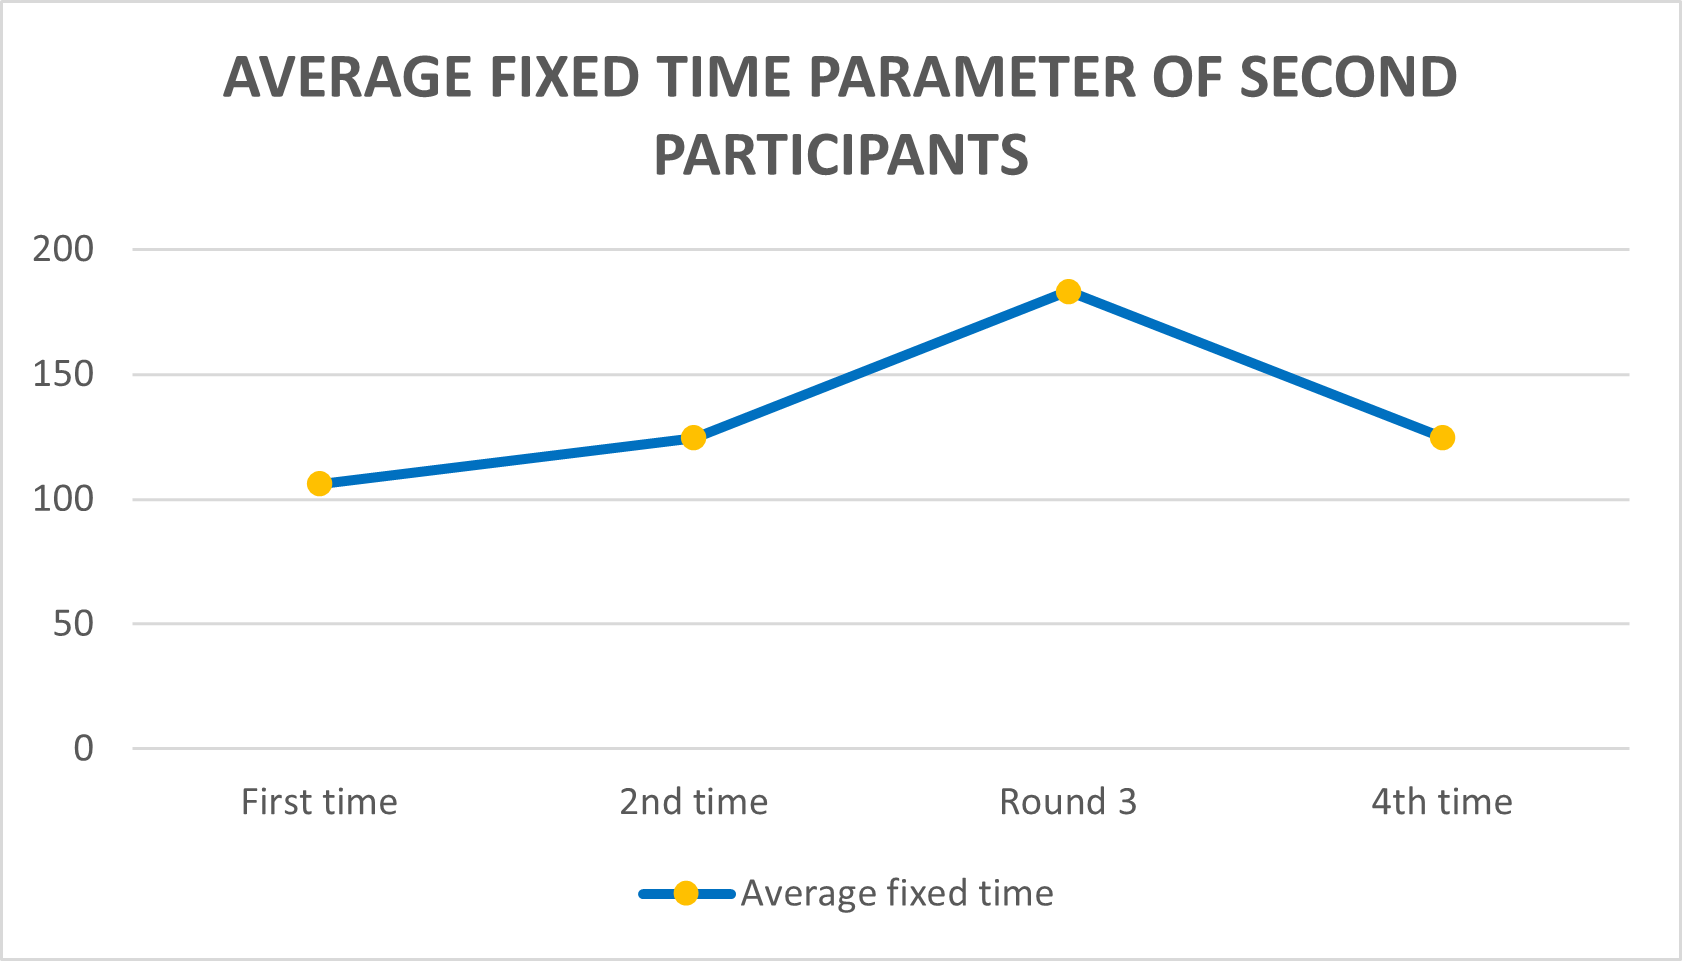
\includegraphics[width=4.1cm]{samples/Data/fig13c.png}\\
        (a) &
        (b)&
        (c)
    \end{tabular}
    \caption{Compare the parameters of the second participant explores on the correct answer rate, the number of frames and the number of fixes (a);total fixed duration (b); and average fixed time (c) in each phase}
    \label{fig14}
\end{figure}

\begin{figure}
    \centering
    \begin{tabular}{cc}
        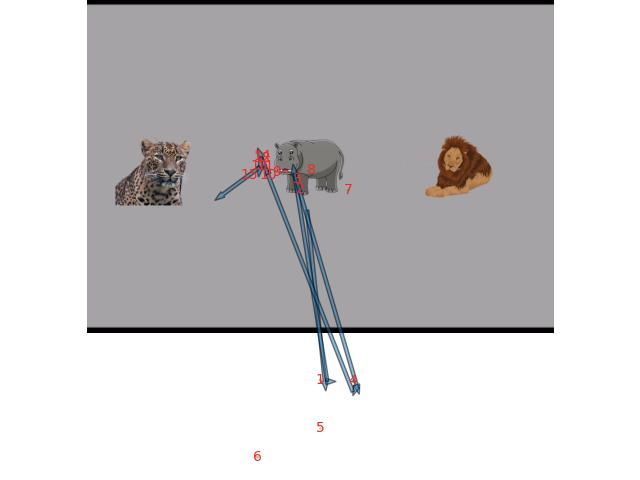
\includegraphics[width=6.5cm]{samples/Data/cycle1b.jpg} &
        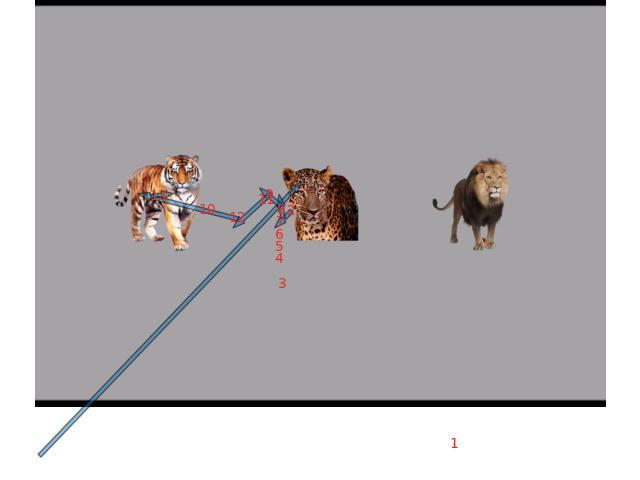
\includegraphics[width=6.5cm]{samples/Data/cycle1c.jpg} \\
        (a) &
        (b)
    \end{tabular}
    \caption{Scanpath of several frames at the baseline time of the 2nd participant}
    \label{figcycle1}
\end{figure}



\subsubsection{Cycle 1: Stabilization:} The system identified this behavior as "Hyper-focus." Consequently, the intervention was adjusted to: (1) provide verbal instructions prior to visual presentation to prime cognitive processing, and (2) remove the "favorite object" distractor during testing phases. Assessment at time 2 showed that exploration expanded to 5 out of 6 frames, and the correct response rate improved to 2 out of 5. However, the participant continued to neglect the right side of the screen, indicating a persistent "blind spot."

\subsubsection{Cycle 2: Load Reduction:} To address the right-side blind spot, the visual load was reduced by decreasing the number of objects per frame to prevent cognitive overload. By Time 3, the correct response rate reached 4 out of 5. The key finding was the child's ability to accurately identify four distinct animal types, demonstrating that conceptual discrimination was no longer dependent on the presence of the "favorite object." Visual attention at the previously neglected "Position 3" (Right) increased to $10\%$, indicating a successful, albeit nascent, expansion of the visual field. The visual illustration of the third participant heatmap and scanpath demonstrates a significant improvement in the field of vision, varying both in the extent of its expansion and the scanning range, from a predominantly vertical scanning tendency to a more flexible horizontal and vertical bidirectional approach.

\begin{figure}
    \centering
    \begin{tabular}{cc}
        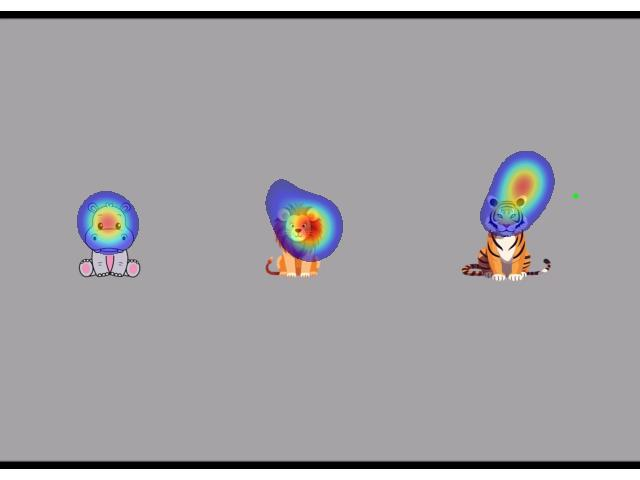
\includegraphics[width=6.5cm]{samples/Data/cycle2a.jpg} &
        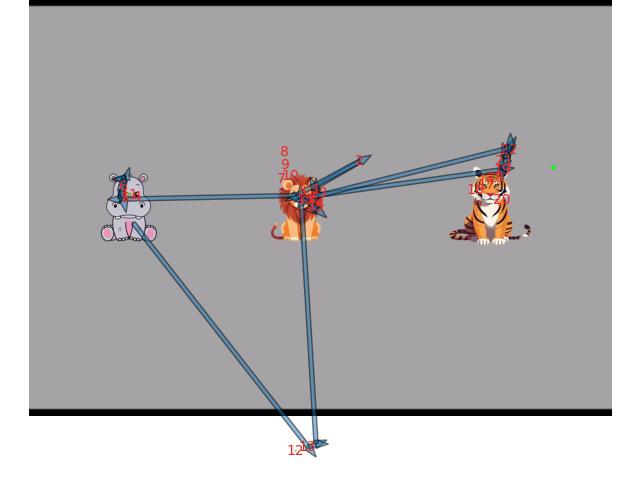
\includegraphics[width=6.5cm]{samples/Data/cycle2b.jpg} \\
        (a) &
        (b)
    \end{tabular}
    \caption{Heatmap and scanpath of a frame at the cycle two time of the 2nd participant}
    \label{figcycle1}
\end{figure}

% \begin{figure}
%     \centering
%     \begin{tabular}{cc}
%         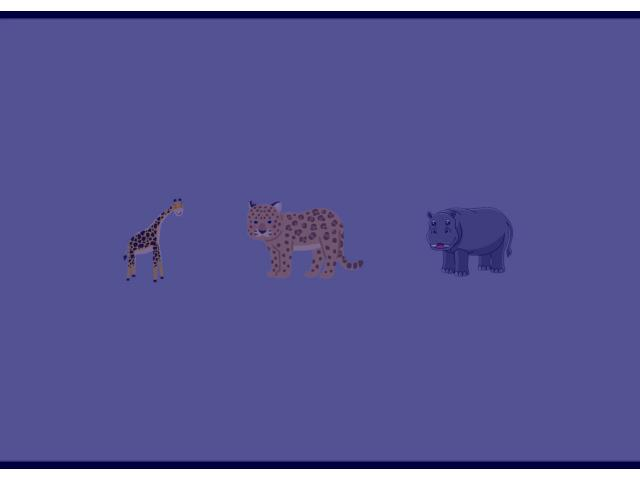
\includegraphics[width=6.5cm]{samples/Data/fig11a.jpg} &
%         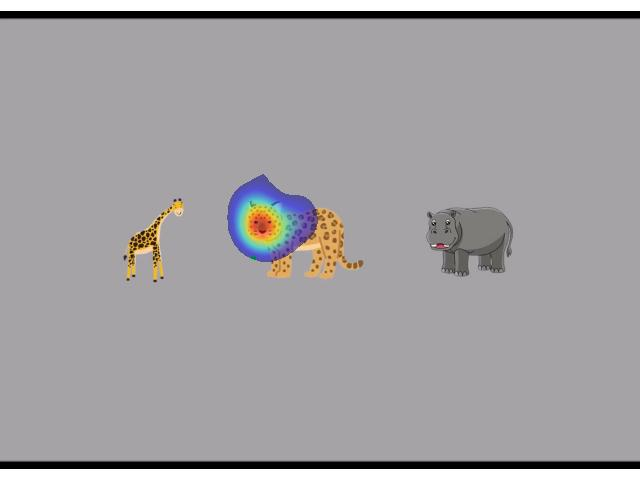
\includegraphics[width=6.5cm]{samples/Data/fig11b.jpg} \\
%         (a) &
%         (b)
%     \end{tabular}
%     \caption{Heatmap of a frame at (a) the baseline and (b) after first intervention times of the 2nd participant}
%     \label{fig12}
% \end{figure}

\subsection{Participant 3: Syntax Construction (PECS phase 4)}
Objective: Sentence structure ("I want" + activity + object).
 Eye-tracking indices for all frames across the four data-collection periods for participant 3 are presented in the table  \ref{tb8}.

 
\begin{tableorg}
        \caption{Eye tracking index for all frames in 4 data acquisitions of participant 3}
        \renewcommand{\arraystretch}{1}
    \centering
    \resizebox{\textwidth}{!}{
    \begin{tabular}{|c|c|c|c|c|}
    \hline
         \parbox{2cm}{\centering\textbf{Measure-\\ment times}}& {\parbox{2cm}{\centering\textbf{Fixed number of times}}} & \parbox{2cm}{\centering\textbf{Fixed duration (ms)}} & {\parbox{2cm}{\textbf{Average fixation duration (ms)}}} & {\parbox{4cm}{\textbf{Ratio of fixed time to total observation time}}}\\ \hline
         1& 213 & 31956 & 150.02 & 45.65\\ \hline
         2& 77 & 9306 & 120.86 &  13.29\\ \hline
         3& 107 & 13402 & 125.25 &  19.15\\ \hline
         4& 104 & 15519 & 149.22 &  22.17\\ \hline
    \end{tabular}
        }
    \label{tb8}
\end{tableorg}

 

 
 
\subsubsection{Baseline analysis (Time 1):} Figure \ref{fig17} presents the eye movement tracking metrics of the second participant over four recordings. Initial scans revealed stochastic viewing patterns. The participant failed to fixate on sentence components in the necessary syntactic order, resulting in fragmented and non-functional communication attempts.

\begin{figure}
    \centering
    \begin{tabular}{ccc}
        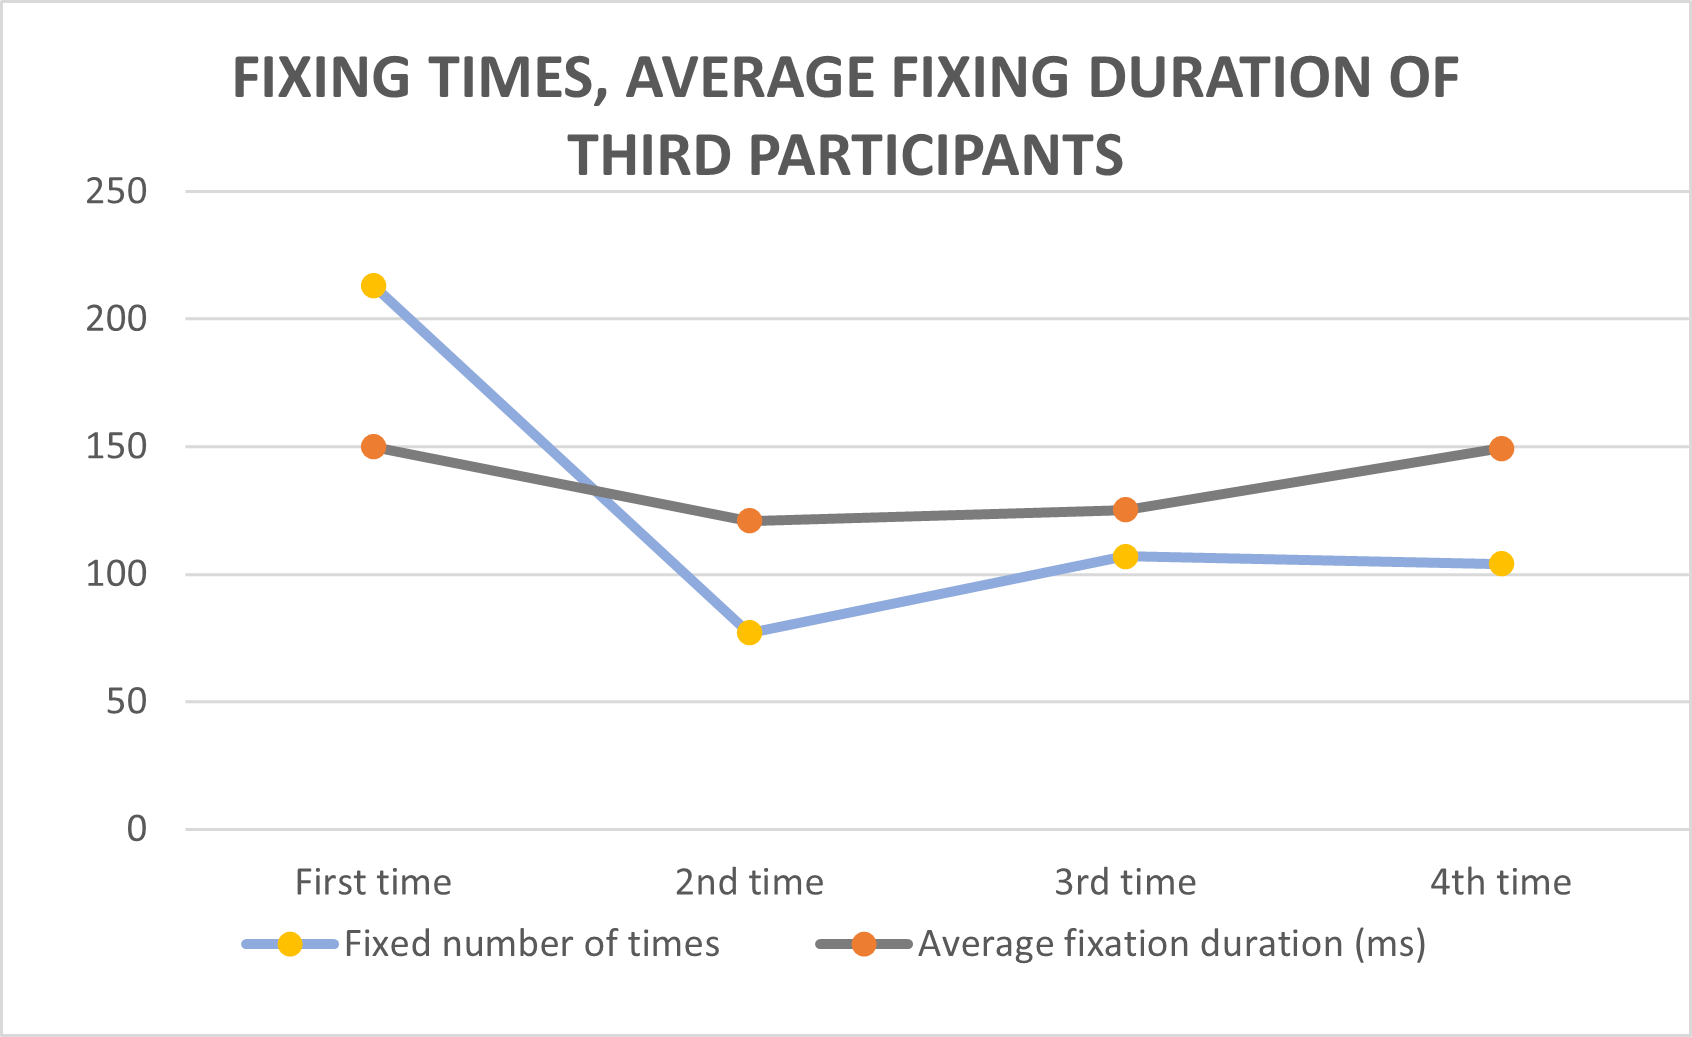
\includegraphics[width=4.1cm]{samples/Data/fig16a.png} &
        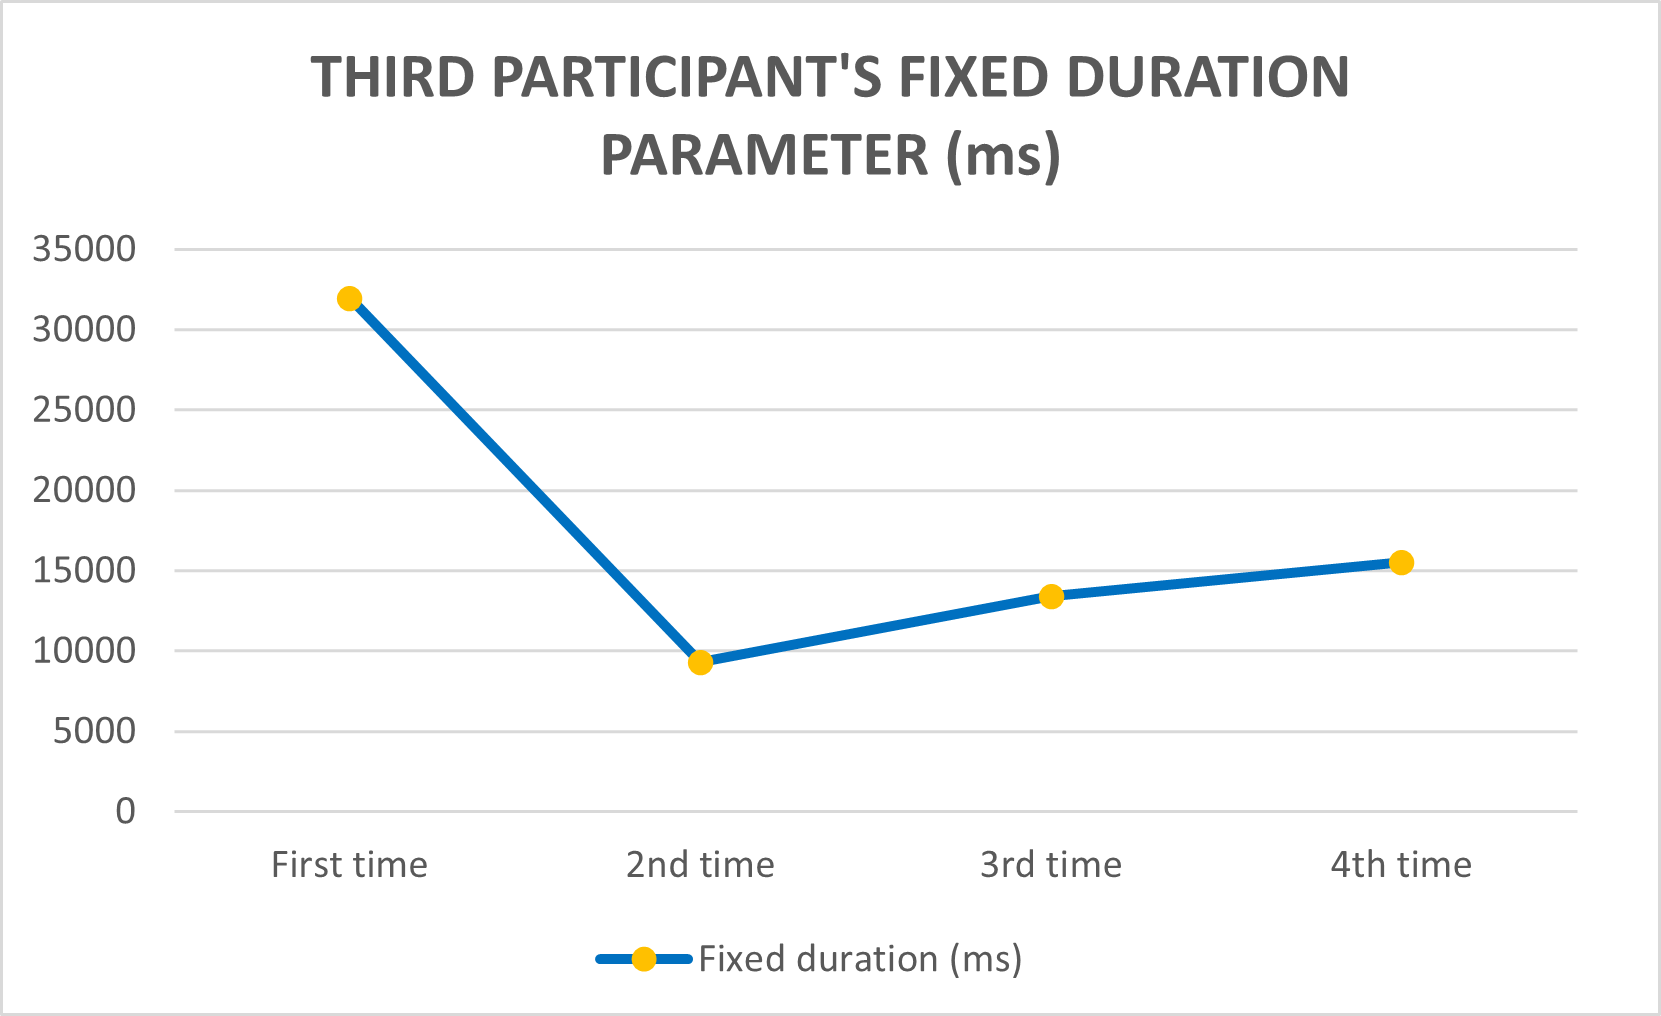
\includegraphics[width=4.1cm]{samples/Data/fig16b.png}&
        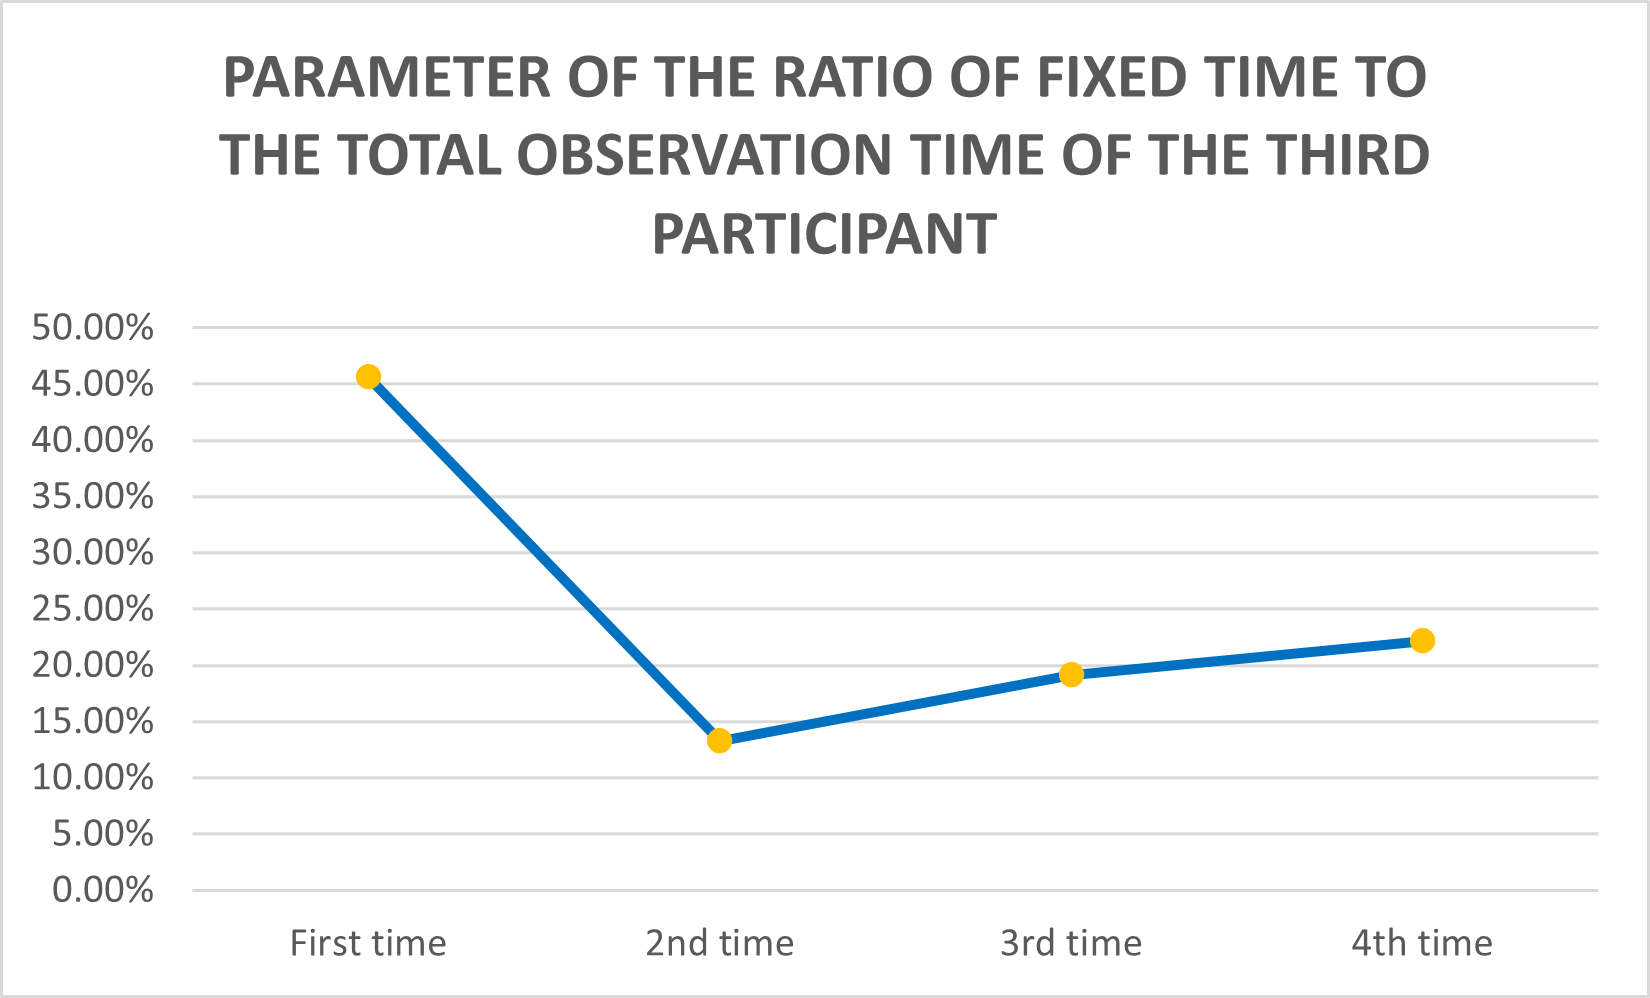
\includegraphics[width=4.1cm]{samples/Data/fig16c.png}\\
        (a) &
        (b)&
        (c)
    \end{tabular}
    \caption{Compare the parameters of the third participant explores on the number of frames and the number of fixes (a);total fixed duration (b); and average fixed time (c) in each phase}
    \label{fig17}
\end{figure}

\begin{figure}
    \centering
    \begin{tabular}{cc}
        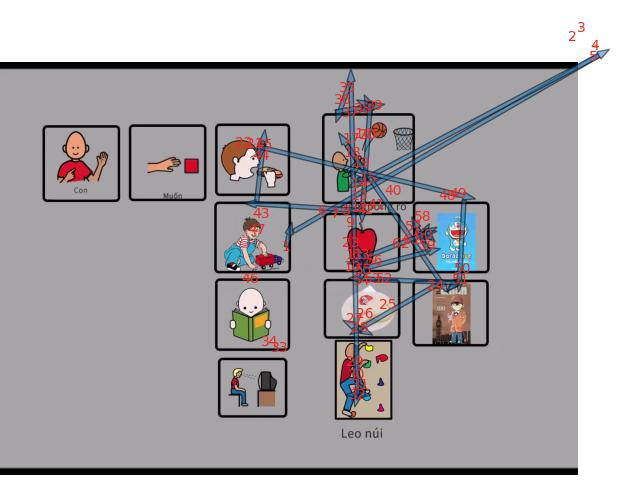
\includegraphics[width=6.5cm]{samples/Data/fig14a.jpg} &
        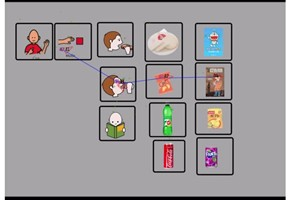
\includegraphics[width=6.5cm]{samples/Data/fig14b.jpg} \\
        (a) &
        (b)
    \end{tabular}
    \caption{Scanpaths of a frame at (a) the baseline and (b) after first intervention times of the 3rd participant}
    \label{fig15}
\end{figure}

\begin{figure}
    \centering
    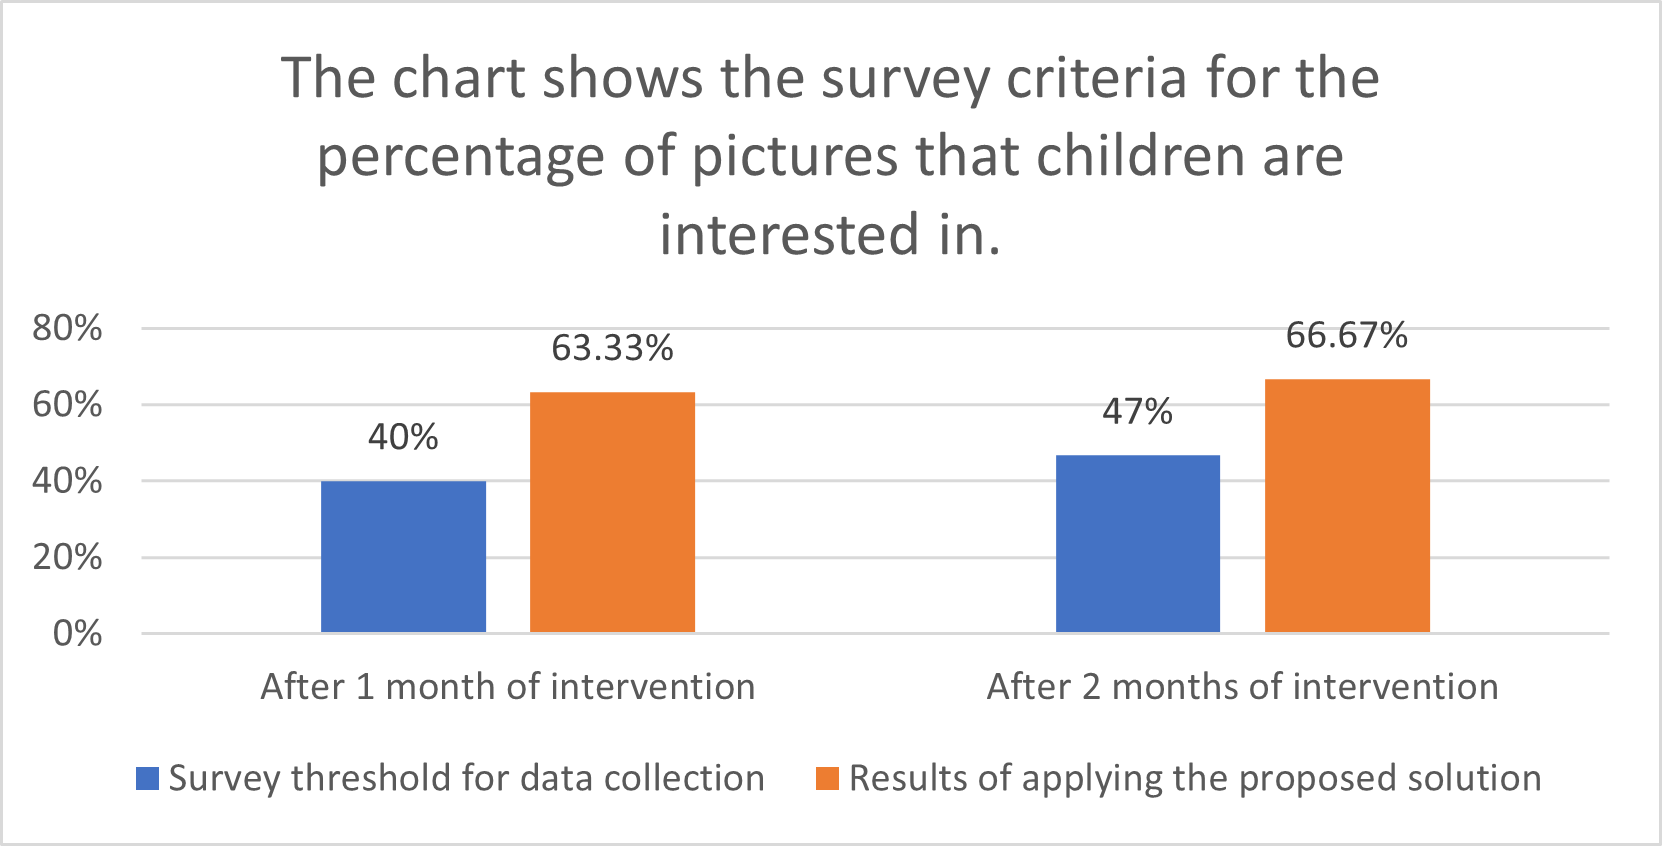
\includegraphics[width=0.9\columnwidth, alt={abc}]{samples/Data/fig19.png}
    \caption{Compare the actual performance level with the expert's prediction based on the first participant's vision (percentage of pictures that children are interested in).}
    \label{fig19}
\end{figure}

\begin{figure}
    \centering
    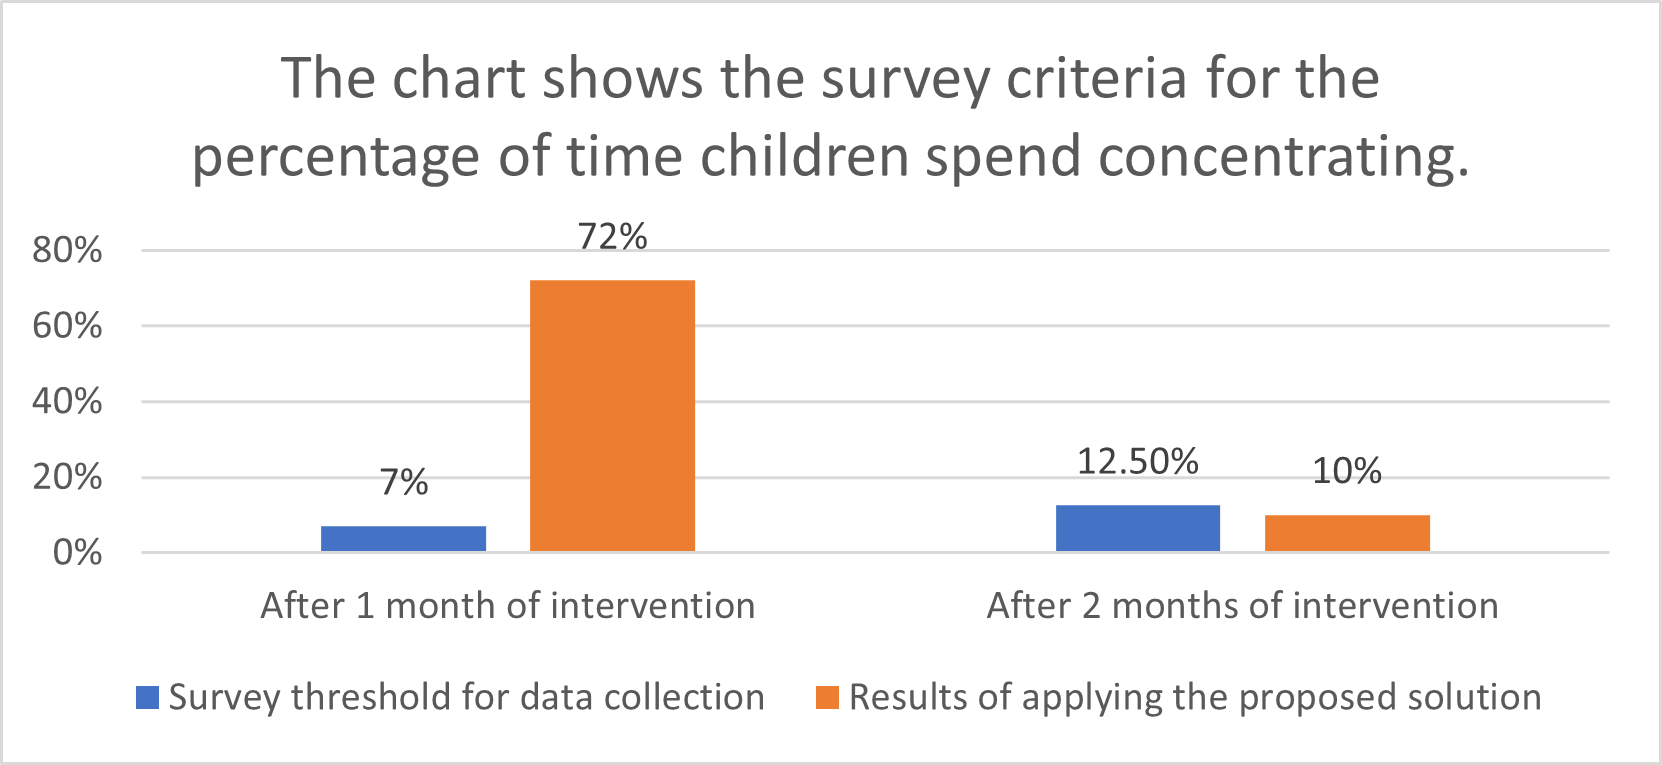
\includegraphics[width=0.9\columnwidth, alt={abc}]{samples/Data/fig20.png}
    \caption{Compare the actual performance level with the expert's prediction based on the first participant's vision (percentage of time children spend concentrating).}
    \label{fig20}
\end{figure}

\begin{figure}
    \centering
    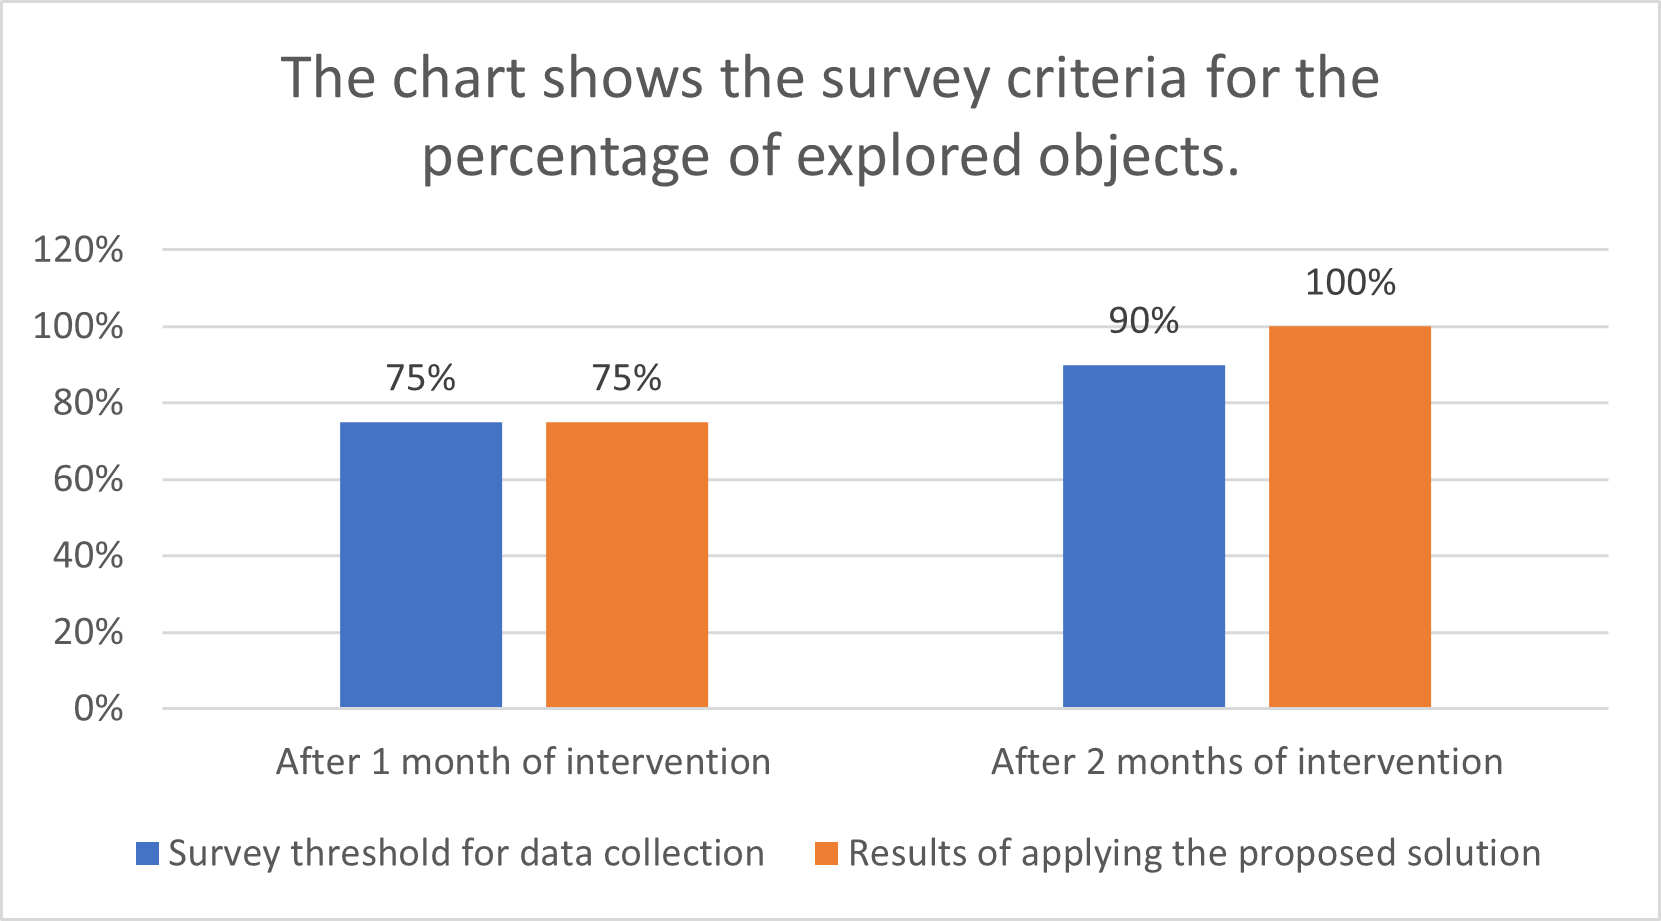
\includegraphics[width=0.9\columnwidth, alt={abc}]{samples/Data/fig21.png}
    \caption{Compare the actual performance level with the expert's prediction based on the first participant's vision (percentage of explored objects).}
    \label{fig21}
\end{figure}

\begin{figure}
    \centering
    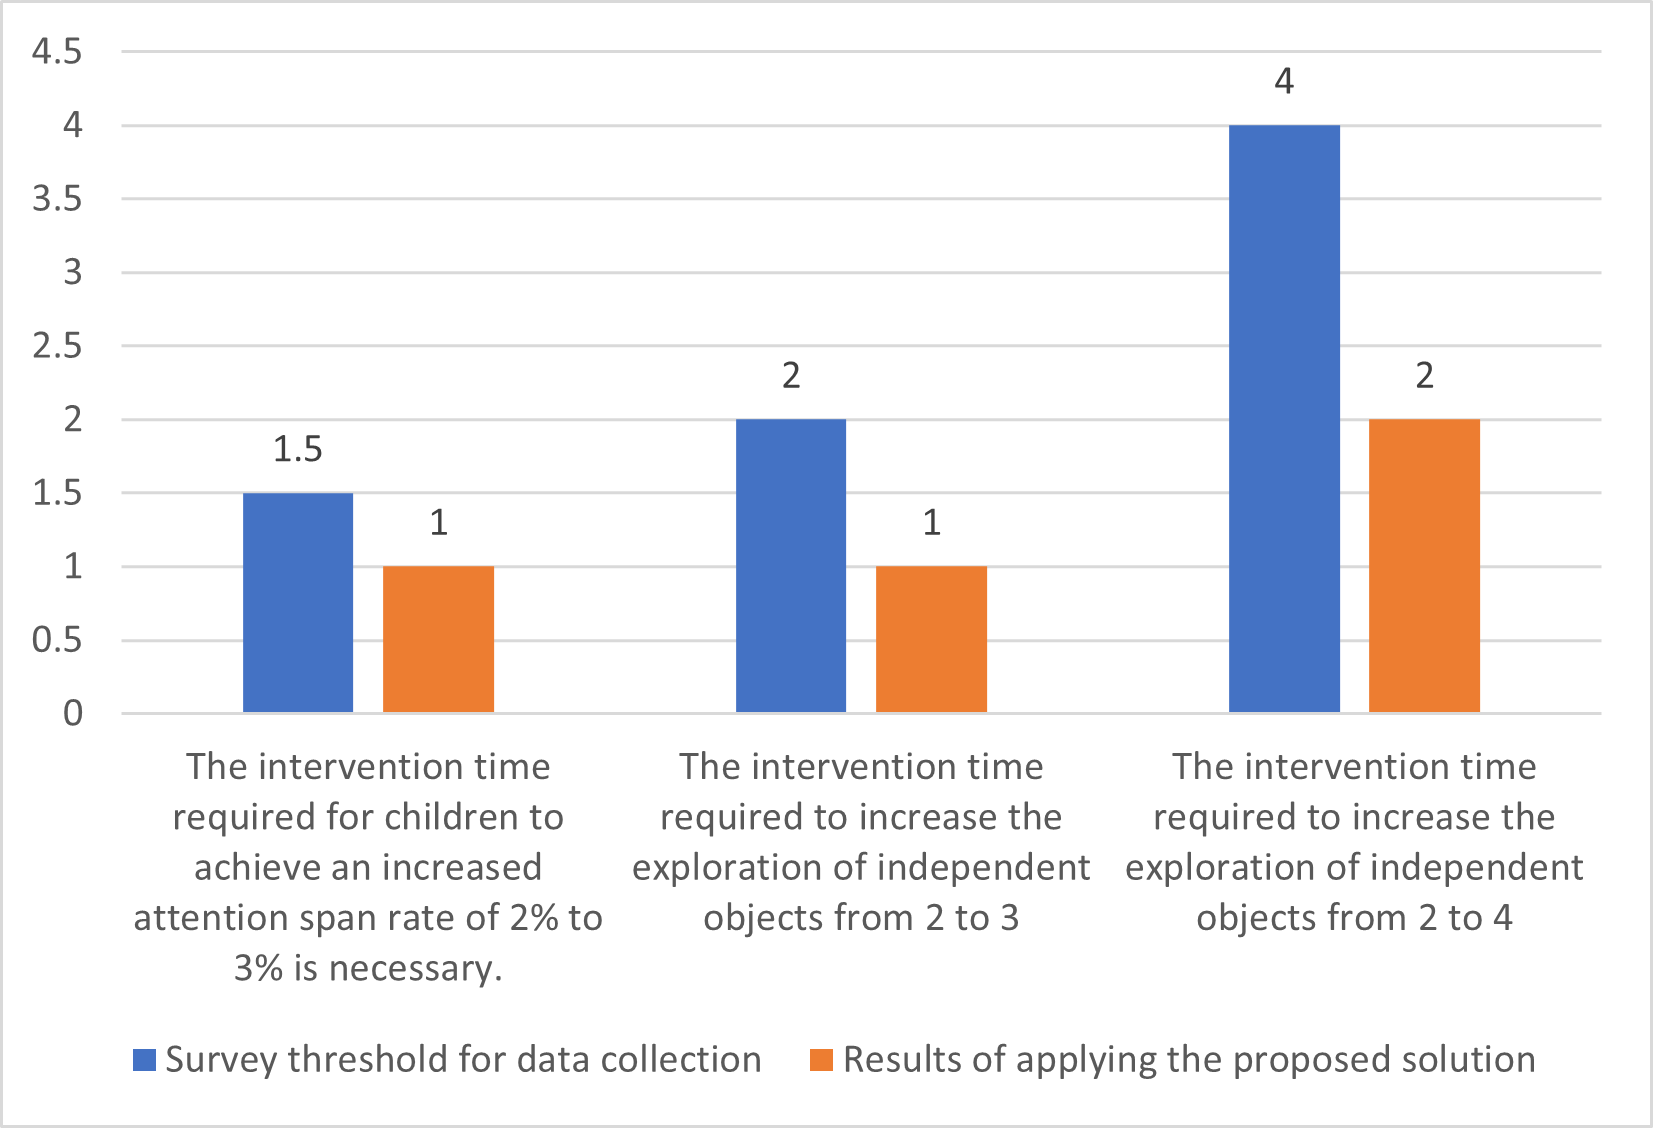
\includegraphics[width=0.9\columnwidth, alt={abc}]{samples/Data/fig9.png}
    \caption{Compare the actual performance duration with the expert's prediction based on the first participant's visual acuity.}
    \label{fig10}
\end{figure}

\begin{figure}
    \centering
    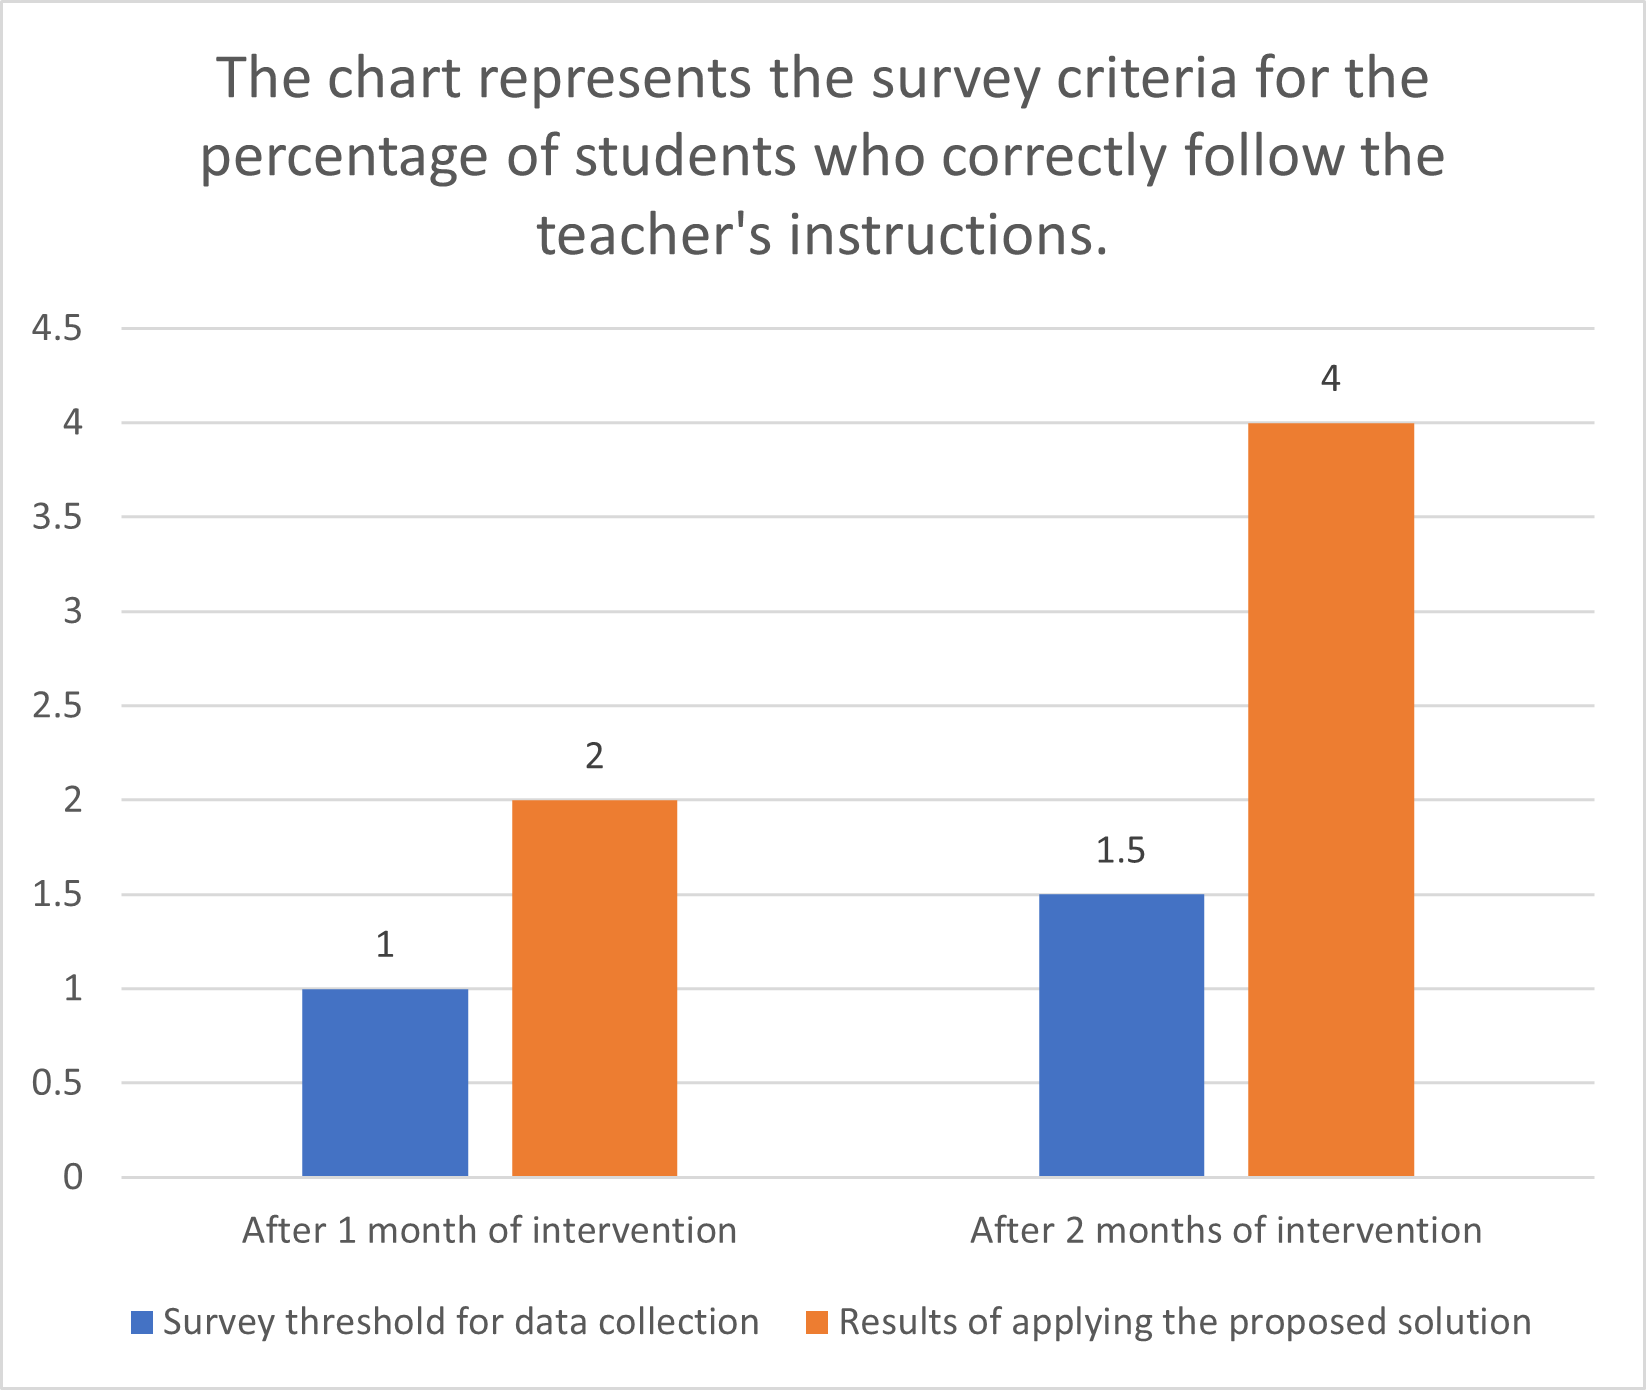
\includegraphics[width=0.9\columnwidth, alt={abc}]{samples/Data/fig18.png}
    \caption{Compare the actual performance level with the expert's prediction based on the second participant's vision.}
    \label{fig18}
\end{figure}

\begin{figure}
    \centering
    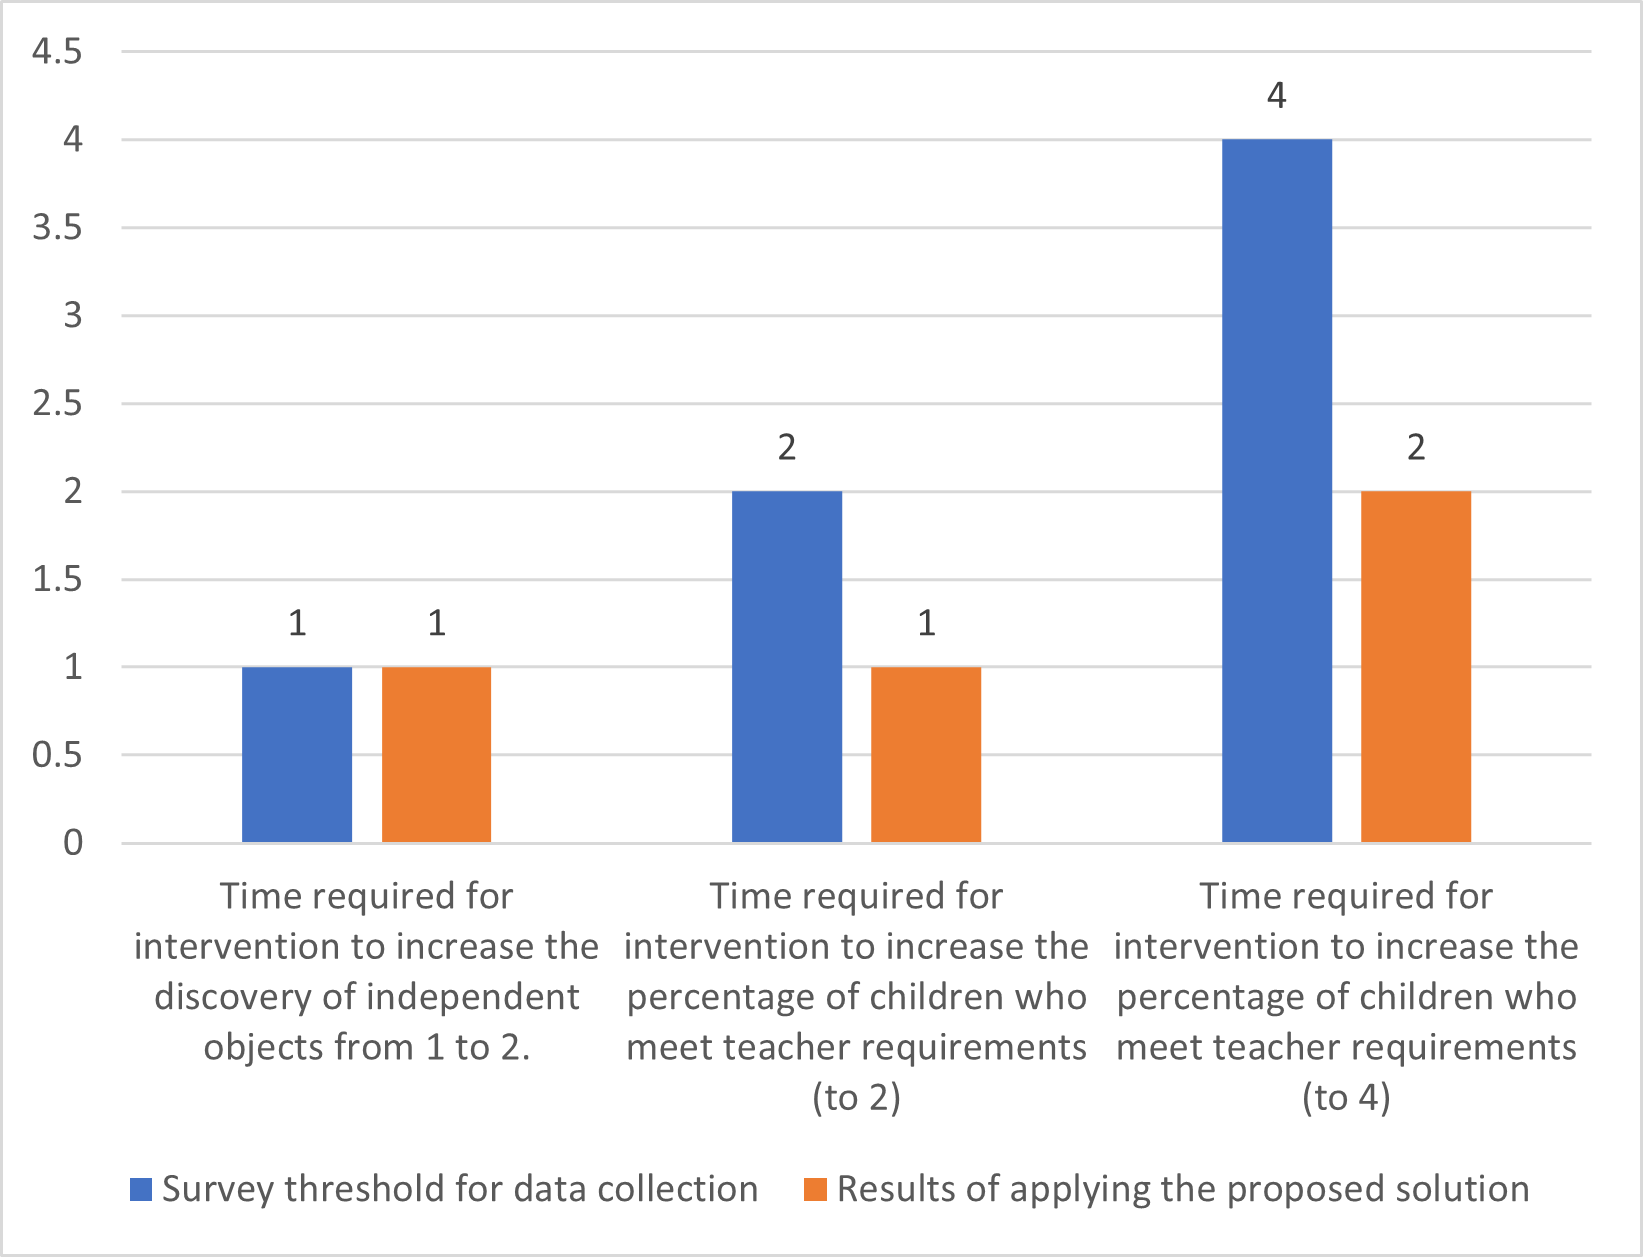
\includegraphics[width=0.9\columnwidth, alt={abc}]{samples/Data/fig12.png}
    \caption{Compare the actual performance duration with the expert's prediction based on the second participant's visual acuity.}
    \label{fig13}
\end{figure}

\begin{figure}
    \centering
    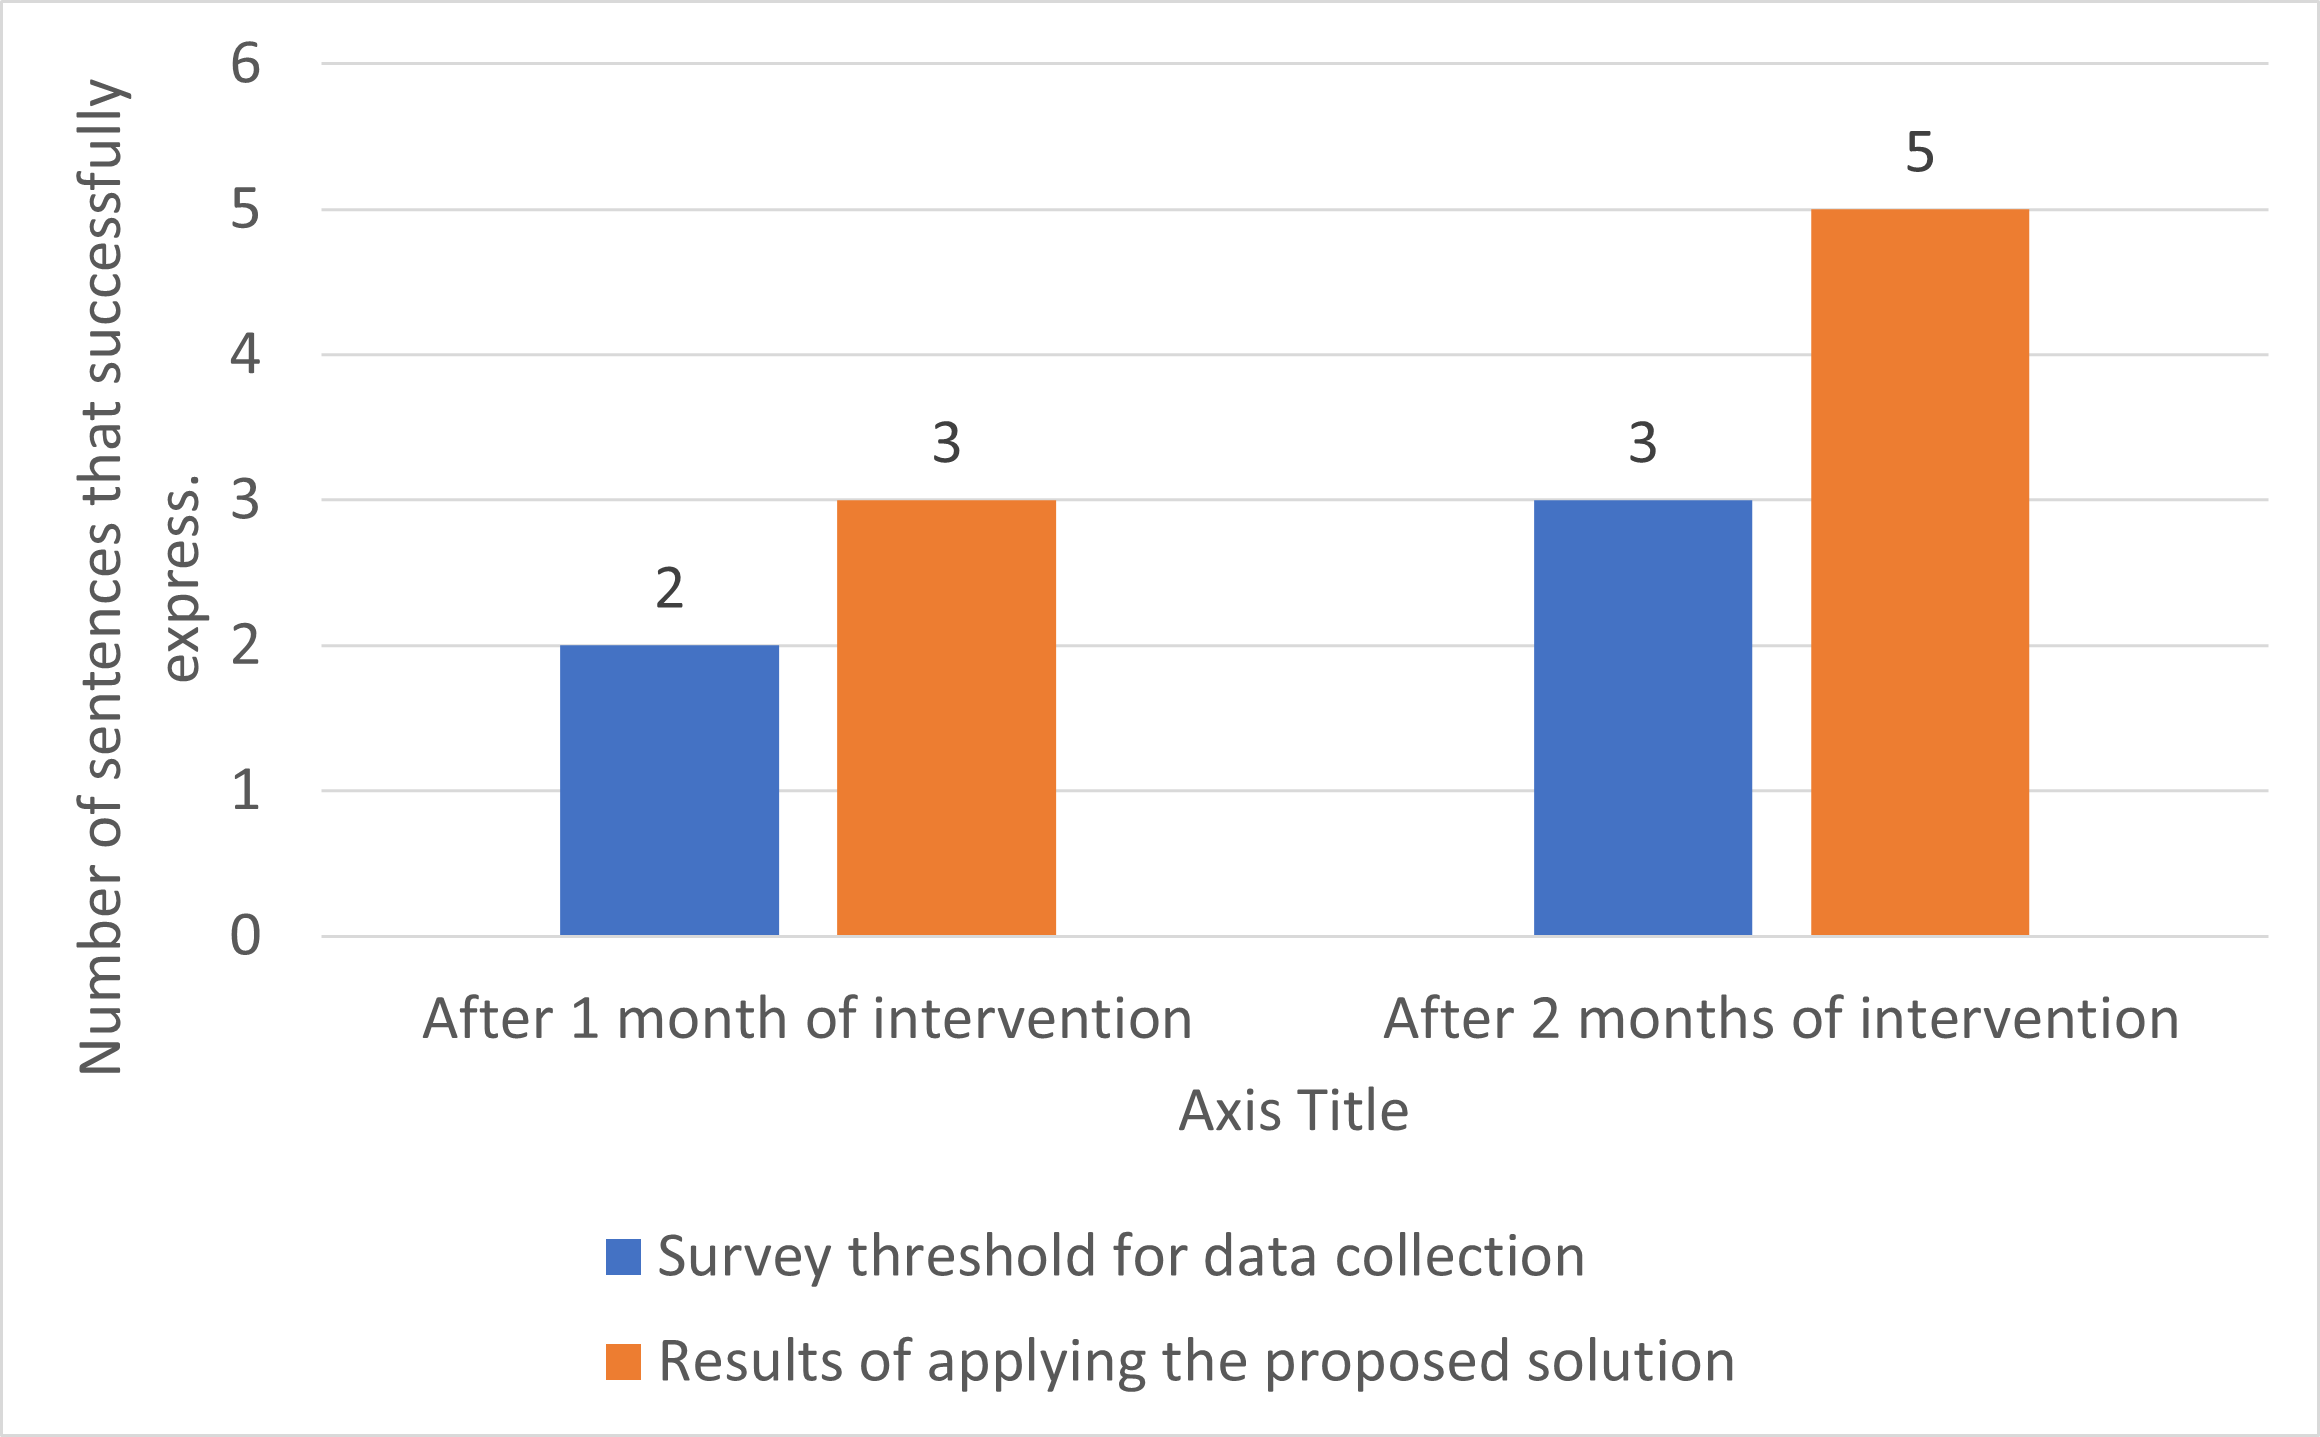
\includegraphics[width=0.9\columnwidth, alt={abc}]{samples/Data/fig17.png}
    \caption{Compare the actual performance level with the expert's prediction based on the third participant's vision.}
    \label{fig17}
\end{figure}

\begin{figure}
    \centering
    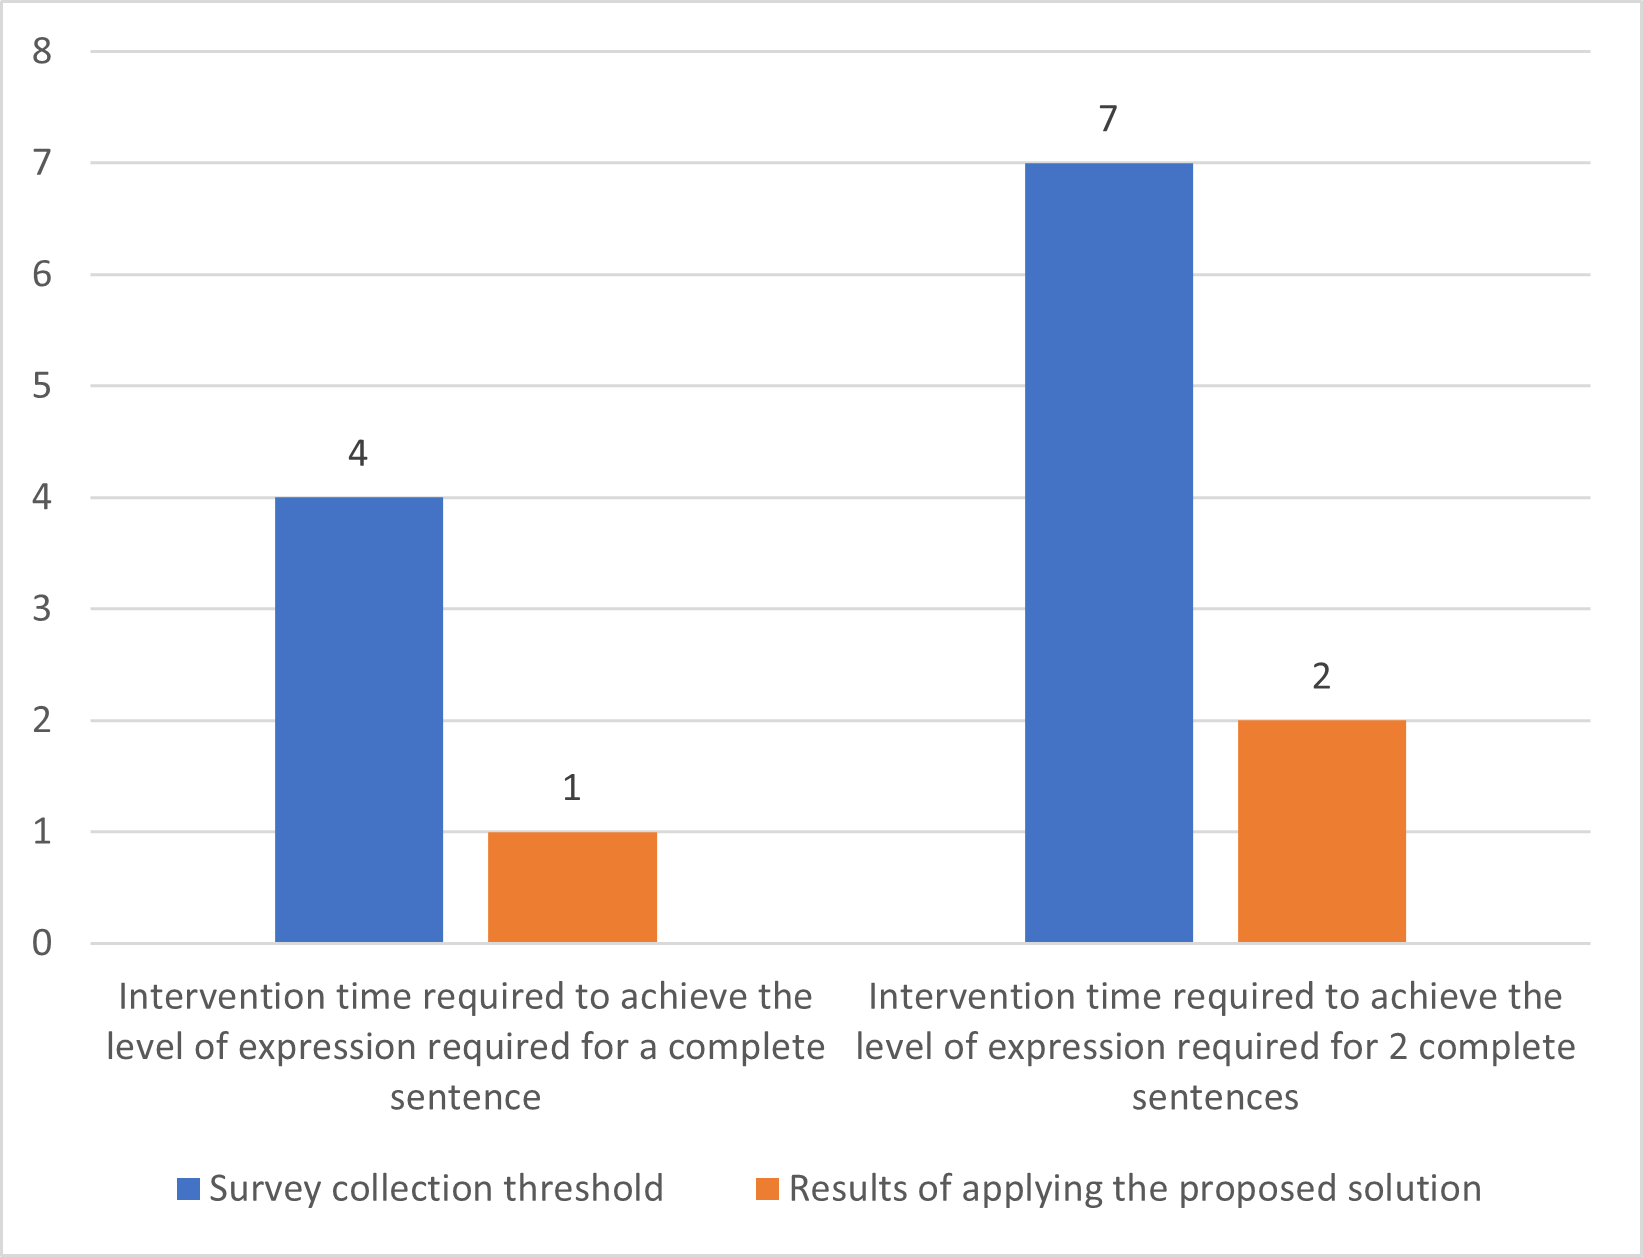
\includegraphics[width=0.9\columnwidth, alt={abc}]{samples/Data/fig15.png}
    \caption{Compare the actual performance duration with the expert's prediction based on the third participant's visual acuity.}
    \label{fig16}
\end{figure}

\subsubsection{Cycle 1: Structuring:} The intervention focused on reducing the array of choices to clarify the fundamental "Subject $\rightarrow$ verb" relationship. This results in a decrease in total fixation count, a positive indicator of increased processing efficiency, and the emergence of the first structured scan paths corresponding to the sequence "I" $\rightarrow$ "want" $\rightarrow$ "activity."

\subsubsection{Cycle 2: Sentence expansion:} The protocol subsequently introduced the "object" slot to complete the sentence structure. By time 3, gaze path analysis confirmed the establishment of a complete linear scan: "I" $\rightarrow$ "want" $\rightarrow$ "activity" $\rightarrow$ "object." Clinically, this visual mastery correlated perfectly with the behavioral ability to construct complete verbal sentences to express desires, bridging the gap between visual attention and linguistic output. Figure \ref{fig15} illustrates the third-person perspective through the scanpath at the baseline and after cycle 2 time, showing a significant change in perspective. Firstly, the visual confusion has been significantly reduced. Secondly, the order of viewing positions is clearer and more coherent, demonstrating the formation of sentences according to the structure of a complete sentence.



\begin{tableorg}
    \caption{Comparison of expert survey results and eye tracking solution application results – subject 1}
    \small
    \label{tb9}
    \renewcommand{\arraystretch}{2.3}
    \centering
    \resizebox{\linewidth}{!}{
    \begin{tabular}{|c|c|c|c|c|c|c|c|}
    \hline
        \multirow{2}{*}{\textbf{No.}} & \multirow{2}{*}{\parbox{1cm}{\textbf{Survey criteria}}} & \multirow{2}{*}{\parbox{1cm}{\textbf{Before intervention}}} & \multicolumn{2}{c|}{\textbf{Survey collection threshold}} & \multicolumn{2}{c|}{\parbox{4cm}{\textbf{Results of applying the proposed solution}}} & \multirow{2}{*}{\parbox{2cm}{\textbf{Evaluation results}}} \\ \cline{4-7}
         &  &  & {\parbox{2.3cm}{After 1 month of intervention}} & {\parbox{2.3cm}{After 2 months of intervention}} & {\parbox{2.3cm}{After 1 month of intervention}} & {\parbox{2.3cm}{After 2 months of intervention}} & \\ \hline
         1& (1) & 16.67 & 40 & 46.67 & 63.33 & 66.67 & \\ \hline
         2& (2) & 2 & 5-10 & 10-15 & 72 & 10 & \\ \hline
         3& (3) & 50 & 75 & 90 & 75 & 100 & \\ \hline
         4& (4) &  & \multicolumn{2}{c|}{1.5 months} & \multicolumn{2}{c|}{1 months} & \\ \hline
         5& (5) &  & \multicolumn{2}{c|}{ 2 month} & \multicolumn{2}{c|}{1 month} & \\ \hline
         6& (6) &  & \multicolumn{2}{c|}{4 months} & \multicolumn{2}{c|}{2 months} & \\ \hline
    \end{tabular}}
    
    \vspace{2mm}
    \parbox{\linewidth}{
    \footnotesize
    \textsuperscript{(1)} Percentage of pictures that children are interested in. \\
    \textsuperscript{(2)} Percentage of time that children concentrate.\\
    \textsuperscript{(3)} Percentage of discovered objects. \\
    \textsuperscript{(4)} The intervention time required for children to achieve a 2 to 3 increase in attention span. \\
    \textsuperscript{(5)} Intervention time required to increase independent object exploration from 2 to 3. \\
    \textsuperscript{(6)} Intervention time required to increase independent object exploration from 2 to 4.}
\end{tableorg}

% (1) Percentage of pictures that children are interested in
% (2) Percentage of time that children concentrate
% (3) Percentage of discovered objects
% (4) The intervention time required for children to achieve a 2 to 3 increase in attention span
% (5) Intervention time required to increase independent object exploration from 2 to 3
% (6) Intervention time required to increase independent object exploration from 2 to 4


\begin{tableorg}
    \caption{Comparison of expert survey results and eye tracking solution application results – subject 2}
    \label{tb10}
    \renewcommand{\arraystretch}{2.3}
    \centering
    \resizebox{\textwidth}{!}{
    \begin{tabular}{|c|c|c|c|c|c|c|c|}
    \hline
        \multirow{2}{*}{\textbf{No.}} & \multirow{2}{*}{\parbox{1cm}{\textbf{Survey criteria}}} & \multirow{2}{*}{\parbox{1cm}{\textbf{Before intervention}}} & \multicolumn{2}{c|}{\textbf{Survey collection threshold}} & \multicolumn{2}{c|}{\parbox{4cm}{\textbf{Results of applying the proposed solution}}} & \multirow{2}{*}{\parbox{2cm}{\textbf{Evaluation results}}} \\ \cline{4-7}
        
         &  &  & {\parbox{2.3cm}{After 1 month of intervention}} & {\parbox{2.3cm}{After 2 months of intervention}} & {\parbox{2.3cm}{After 1 month of intervention}} & {\parbox{2.3cm}{After 2 months of intervention}} & \\ \hline
         1& (1) & 16.67 & 25 & 30 & 83.33 & 83.33 & \\ \hline
         2& (2) & 0.22 & 1 & 2 & 2.25 & 4 & \\ \hline
         3& (3) & 0 & 1 & 1.5 & 2 & 4 & \\ \hline
         4& (4) & 1 & 2 & 4 & 4 & 4 & \\ \hline
         5& (5) &  & \multicolumn{2}{c|}{Over 1 month} & \multicolumn{2}{c|}{Under 1 month} & \\ \hline
         6& (6) &  & \multicolumn{2}{c|}{2 months} & \multicolumn{2}{c|}{1 months} & \\ \hline
         7& (7) &  & \multicolumn{2}{c|}{4 months} & \multicolumn{2}{c|}{2 months}  & \\ \hline
    \end{tabular}
    }
    
    \vspace{2mm}
    \parbox{\linewidth}{
    \footnotesize
    \textsuperscript{(1)} Percentage of pictures that children are interested in. \\
    \textsuperscript{(2)} Percentage of time that children concentrate.\\
    \textsuperscript{(3)} Rate of correct implementation of teacher's requirements. \\
    \textsuperscript{(4)} Number of discovered objects. \\
    \textsuperscript{(5)} Intervention time required to increase independent object exploration from 1 to 2. \\
    \textsuperscript{(6)} Intervention time required to increase the proportion of children who correctly performed teacher requests (by 2). \\
    \textsuperscript{(7)} Intervention time required to increase the proportion of children who correctly performed teacher requests (by 4).}
\end{tableorg}

% (1) Percentage of pictures that children are interested in.
% (2) Percentage of time that children concentrate.
% (3) Rate of correct implementation of teacher's requirements.
% (4) Number of discovered objects.
% (5) Intervention time required to increase independent object exploration from 1 to 2.
% (6) Intervention time required to increase the proportion of children who correctly performed teacher requests (by 2).
% (7) Intervention time required to increase the proportion of children who correctly performed teacher requests (by 4).




\nopagebreak
\begin{tableorg}
    \small
    \caption{ Comparison of expert survey results and eye tracking solution application results – participant 3}
    \label{tb11}
    \renewcommand{\arraystretch}{3}
    \centering
    \resizebox{\textwidth}{!}{
    \begin{tabular}{|c|c|c|c|c|c|c|c|}
    \hline
        \multirow{2}{*}{\textbf{No.}} & \multirow{2}{*}{\parbox{1cm}{\textbf{Survey criteria}}} & \multirow{2}{*}{\parbox{1.5cm}{\textbf{Before intervention}}} & \multicolumn{2}{c|}{\textbf{Survey collection threshold}} &  \multicolumn{2}{c|}{\parbox{4cm}{\textbf{Results of applying the proposed solution}}}  & \multirow{2}{*}{\parbox{2cm}{\textbf{Evaluation results}}}\\ \cline{4-7}
         &  &  & {\parbox{2.3cm}{After 1 month of intervention}} & {\parbox{2.3cm}{After 2 months of intervention}} & {\parbox{2.3cm}{After 1 month of intervention}} & {\parbox{2.3cm}{After 2 months of intervention}} & \\ \hline
         1& (1) &0.5 sentence & 2 sentence & 3 sentence & 3 sentence & 5 sentence &   \\ \hline
         2& (2) &  & \multicolumn{2}{c|}{4 months} & \multicolumn{2}{c|}{1 month} &   \\ \hline
         3& (3) &  & \multicolumn{2}{c|}{7 months} & \multicolumn{2}{c|}{2 months} & \\ \hline
    \end{tabular}
        }
    
    \vspace{2mm}
    \parbox{\linewidth}{
    \footnotesize
    \textsuperscript{(1)} Number of desired expressions of success.\\
    \textsuperscript{(2)} Intervention time required to achieve the level of expression required for a complete sentence.\\
    \textsuperscript{(3)} Intervention time required to achieve the level of expression required for 2 complete sentences. \\ }
\end{tableorg}

% (1) Number of desired expressions of success
% (2) Intervention time required to achieve the level of expression required for a complete sentence
% (3) Intervention time required to achieve the level of expression required for 2 complete sentences
\nopagebreak


\subsection{Comparative validation: Actual outcomes vs. expert predictions}
Comparative Validation Analysis
To empirically validate the clinical efficiency of the proposed framework, actual intervention outcomes were juxtaposed against predictive benchmarks established by a cohort of 31 domain experts (see table \ref{tb2}). This comparative analysis encompassed a total of 18 performance criteria, distributed as six distinct metrics per participant. The evaluation focused on two primary dimensions: Projected proficiency (Magnitude), defined as the estimated level of skill improvement achievable within a standard 1–2 month clinical window without ET support; and time to acquisition (Velocity), defined as the projected duration required for the child to reach specific therapeutic milestones under standard care.
Detailed quantitative results for the three participants are stratified in tables \ref{tb9}, \ref{tb10}, and \ref{tb11}. These comparisons are visually represented in figures \ref{fig19} - \ref{fig16}, which contrast the expert prediction (Left column) directly with the actual ET-assisted outcome (Right column). A granular analysis of participant 3 reveals a notable divergence between prediction and reality, particularly regarding communicative output. While the expert consensus forecasted only a modest increase in sentence production after one month, the actual outcomes facilitated by the framework's syntax scaffolding significantly exceeded these conservative estimates. Furthermore, regarding time to acquisition, the ET-assisted intervention enabled the participant to achieve mastery with substantially reduced latency compared to the timeline projected by experts based on the child's historical clinical records.



\nopagebreak
\begin{tableorg}
    
    \caption{Expert survey criteria for each intervention target}
    \label{tb2}
    \centering
    \resizebox{\textwidth}{!}{
    \begin{tabular}{|c|p{11cm}|c|c|c|}
        \hline
        \multirow{2}{*}{\textbf{No.}} & \multirow{2}{*}{\textbf{Survey Criteria}} & \multicolumn{3}{c|}{\textbf{Participant}} \\ \cline{3-5} 
        & & \textbf{1st} & \textbf{2nd} & \textbf{3rd} \\ \hline
        1 & Percentage of pictures that children are interested in & x & x & \\ \hline
        2 & Percentage of time that children concentrate & x & x & \\ \hline
        3 & Percentage of discovered objects & x & x & \\ \hline
        4 & The intervention time required for children to achieve a 2 percent to 3 percent increase in attention span & x & x & \\ \hline
        5 & Intervention time required to increase independent object exploration from 2 to 3 & x & x & \\ \hline
        6 & Intervention time required to increase independent object exploration from 2 to 4 & x & x & \\ \hline
        7 & Number of desired expressions of success &  &  & x\\ \hline
        8 & Intervention time required to achieve the level of expression required for a complete sentence &  &  & x\\ \hline
        9 & Intervention time required to achieve the level of expression required for 2 complete sentences & & & x \\ \hline
    \end{tabular}
        }
\end{tableorg}
\nopagebreak

 The results indicated that in 15 criteria ($83\%$), the participants performed better or achieved goals faster than predicted by the expert panel. Two criteria showed performance equivalent to predictions, and only one criterion fell below the predicted trajectory. These findings strongly suggest that the integration of the ET-based framework significantly accelerates skill acquisition compared to the expected trajectory of traditional, manual interventions.




































\section{Discussions}
\subsection{Interpretation of main results: bridging oculometrics and cognition}

Following the intervention, quantitative analysis of the oculometric data revealed substantial and positive modifications in the participants' attentional topography. Specifically, the observed increase in fixation duration within semantic AOIs, coupled with the optimization of scanpaths, reflected a fundamental cognitive shift: participants transitioned from a state of distributed, chaotic information processing to a focused strategy targeting the core features of the visual stimulus.

These results underscore the critical utility of objective visual data, not merely for retrospective assessment, but for the active development of individualized therapeutic strategies. By analyzing granular metrics, such as fixation density and saccadic trajectories, the framework successfully isolated the precise nature of a child's difficulties, effectively distinguishing between sensory and cognitive deficits. For instance, in the case of participant 1 (PECS phase 3), a failure to choose the correct card might traditionally be misattributed to non-compliance or a lack of cognitive understanding. However, the eye-tracking (ET) data elucidated that the failure was strictly visual in origin, specifically a left-side lateral bias ($66.67\%$ concentration). This objective insight allowed for a targeted "Accommodation strategy," which successfully neutralized the bias and expanded visual coverage to $100\%$ by Time 3.
Furthermore, the data provided a physiological correlate to language acquisition, as evidenced by participant 3. The transition from stochastic scanning to a linear scanpath ("I" $\to$ "want" $\to$ "object") demonstrates that gaze behavior serves as a reliable proxy for syntactic planning, confirming that the system can detect the emergence of cognitive structures before they are fully verbalized. Consequently, this study confirms the dual role of ET technology: first, as a rigorous measurement tool for quantifying the "semantic gap" between instruction and reception; and second, as a real-time clinical support system. The capacity to detect visual processing barriers at the onset allows interventionists to execute immediate, evidence-based adjustments, such as simplifying visual complexity or employing gaze-contingent cues—thereby effectively closing the feedback loop within the intervention cycle.

\subsection{Efficacy against expert consensus}
A pivotal finding of this study is the demonstrated superiority of data-driven decision-making over traditional clinical intuition. In the comparative analysis, the ET-integrated intervention enabled participants to achieve goals faster or with higher proficiency than predicted by a panel of 31 domain experts across 15 of 18 criteria (an 83\% success rate). This discrepancy suggests that human observation, while empathetic, often underestimates a child's learning velocity when subtle sensory barriers, such as the "Attentional tunnelling" observed in participant 2, remain invisible. The framework acts as a force multiplier, revealing these invisible barriers and facilitating micro-adjustments that human intuition alone cannot calibrate.

\subsection{Implications for practice and research}
This research holds significant dual implications for both clinical practice and the trajectory of scientific inquiry in special education. In practice, the framework provides educators and therapists with a powerful diagnostic lens, shifting the field from subjective estimation to evidence-based decision-making. The ability to visualise a child’s cognitive processes through objective data facilitates deep personalisation of teaching protocols, significantly reducing the duration of interventions for foundational skills by ensuring strategies align with the child's physiological attentional capacity. Scientifically, this research demonstrates a successful bridge between basic cognitive science, specifically oculomotor research, and applied intervention science. It shifts the paradigm of ET from a passive descriptive instrument to an active, integrated component of the therapeutic problem-solving loop. Furthermore, the establishment of objective outcome indicators relying on visual features enriches traditional behavioural assessments, opening new avenues for defining and measuring "progress" in ASD research.

\subsection{Limitations}
While the results are promising, several limitations must be acknowledged to contextualize the findings. First, the study employed a single-subject experimental design with a small sample size ($N=3$) and lacked a control group. While appropriate for determining feasibility and establishing proof-of-concept, this limits the ability to establish broad causal relationships or definitively rule out confounding factors such as natural maturation or the novelty effect of the equipment. Second, regarding ecological validity, the intervention was conducted in a tightly controlled, screen-based setting, limiting the generalization of findings to naturalistic, dynamic environments where social interactions are unpredictable and three-dimensional. Finally, the practical implementation of this framework faces barriers regarding the cost of high-frequency ET hardware and the requirement for specialized personnel to interpret the data, potentially limiting widespread applicability in under-resourced settings.

\subsection{Future Research}
Future research should prioritize four key areas to address these limitations and expand the potential of this approach. First, rigorous validation via RCTs with larger cohorts is urgently needed to statistically establish the causal link between ET-integrated intervention and behavioral progress. 

Second, studies should investigate generalization to natural contexts to determine whether visual attention skills trained on-screen transfer to real-world interactions. This implies the necessity of using wearable ET glasses to monitor gaze patterns during face-to-face family interactions or classroom activities.

Third, the model should be explored for complex social skills, moving beyond static object discrimination to higher-order targets such as interpreting facial expressions and maintaining joint attention during conversation. Finally, to improve clinical viability, research must focus on automation and accessibility. Developing low-cost solutions, such as webcam-based gaze estimation using machine learning, and building intelligent systems that can automate the "Rule-based system" analysis to provide real-time recommendations, would represent a breakthrough in reducing the professional workload.


\section{Conclusion}
This study presents and validates a novel eye-tracking-based framework for intervention efficacy, effectively addressing the critical lack of objective monitoring tools in the treatment of ASD. By transforming the "Observation and adjustment" phase of the therapeutic cycle from a subjective art into a quantitative science, the framework provides clinicians with the insights needed to personalize care effectively.

The experimental application demonstrated that it is technically feasible to map raw oculometric data to meaningful clinical goals (PECS, ABLLS-R). More importantly, data-driven adjustments led to accelerated skill acquisition that outperformed expert predictions in $83\%$ of evaluated criteria. Furthermore, the Maintenance Phase results confirm that these improvements are not merely artifacts of the technology but represent sustained behavioral learning. In conclusion, this research confirms that eye-tracking is not merely a research instrument but a viable, active component of clinical intervention. By making the invisible cognitive processes of children with ASD visible, we empower therapists to make precise, evidence-based decisions that significantly optimize educational outcomes.

\section*{Declarations}
\begin{itemize}
    \item \textbf{Funding:} This research received no specific grant from any funding agency in the public, commercial, or not-for-profit sectors.
    \item \textbf{Conflict of interest: } The authors declare no conflict of interest.
    \item \textbf{Ethics approval: }All procedures performed in studies involving human participants were in accordance with the ethical standards of the institutional and/or national research committee and with the 1964 Helsinki Declaration and its later amendments or comparable ethical standards. The study was approved by the Ethics Committee of Hanoi University of Education.
    \item \textbf{Consent to participate: }Informed consent was obtained from all individual participants included in the study.
    \item \textbf{Consent to publish: }Not applicable.
    \item \textbf{Code availability: } Not applicable.
    \item \textbf{Availability of data and materials: }Not applicable.
\end{itemize}



\bibliography{sn-bibliography}% common bib file
%% if required, the content of .bbl file can be included here once bbl is generated
%%\input sn-article.bbl

\end{document}
